\documentclass[10pt,a4paper]{article}
\usepackage[latin1]{inputenc}
\usepackage{amsmath}
\usepackage{amsfonts}
\usepackage{amssymb}
\usepackage{enumitem}
\usepackage{graphicx}
\usepackage{mathtools}
\usepackage{framed}
\usepackage[numbers]{natbib}


%opening
\title{Evolution of metabolic networks}
\author{Balint Borgulya}

\begin{document}
	
	
	
	\maketitle
	
	\begin{abstract}
		
	\end{abstract}
	
	\section*{TODO}
	\label{sec:todo}
	
	Multiple sources - Programmed
	Multiple sinks - Programmed

	Different goal (biomass production also) ON IT'S WAY - Programmed

	Horizontal gene transfer --- done simulations on the way

	6 carbon CHOPN not happening --- remove from mentions

	Definitions in footnotes? - > in a box. Can't really do two columns - Appendix? smaller text at least font 9

	Are the current compounds really 3 carbon??? There's many that have 4 carbon

	Similarity matrix (partilly done)

	Entropy (kindof done) - Inverse participation ratio  IPR find a citation

	Extract of the data files fullnewreaction.dat and fullnewcompounds.dat into appendix

	EMP ED pathways and the trunk of the glycolytic pathway - how are they related below above ?

	More about biological evolution in intro - 1-2 sentences about it's importance

	More simulations with different concentrations?

	WHERE IS THE PHYSICS PART --- partially okay, need to iterate a few times

	color real glycolysis in the networks shown!!!

	Personal statement

	\newpage
	\section*{Personal statement}
	I spent the first two weeks reading literature suggested by my supervisor, and getting familiar with C++, as I was not familiar with it before. 
	I started developing the simulation software in early October, I received initial help and advice from my friend familiar with C++, who helped me resolving bugs throughout the project. 

	I originally used the Boost graph library to store the reaction network, using this I could simulate simple trial networks at the end of October. It became apparent then that the functionality provided by Boost comes at a large performance cost, so in the first few weeks of November I changed the program to use vectors instead of the Boost concepts. I later implemented a pre-calculation of the reaction neighbour-list substantially speeding up the calculation. 
	In the last week of November I implemented outputting the reaction networks into the XGMML file format that Cytoscape can read for visualisation of the networks. 

	Over the winter break I attempted creating an algorithm that would execute a Depth first search through all reactions in order to find alternative pathways to start the MN from, unfortunately this was very ineffective, so I used a subsection of normal glycolysis as the initial network. Over the break I also read articles in the field and I started drafting the report itself. 

	In January I started running the first simulations with the modified trunk of the glycolytic pathway as the initial network. I also implemented the scripts necessary to perform parallel simulations on multiple computers in the physics cplab, and collecting the results of them. 
	As the simulation results started to flow in, I started to create analysis tools for them, plotting relevant quantities. The log file the simulation outputs while running changed and expanded during this time. 

	In February I implemented an index-based population, where instead of 100 metabolic networks I only store 100 references to types of metabolic networks. This was a performance boost for the simulations with a low mutation rate, as the iterations when no mutations happened could be calculated nearly instantly, since the flux balance analysis problem wasn't necessary to solve in these cases. 

	In February and March I run into problems with the IT infrastructure at the simulating machines, slowing down the progress. I have also had simulations that were started with bad parameters. These errors were fixed when discovered. 

	I started writing the report in January, and worked on it continuously, however the majority of the work on it was done in March. 

	The project's github page REFERENCE and the commit history there serves as diary of the project. 
	\newpage
	\section*{Definitions put it in a box}

	\begin{framed}

	Metabolite: a chemical compound produced in the metabolic network

	Nutrient: chemical compound(s) a cell consumes in order to provide itself with energy and materials.

	Enzyme:

	ATP - Adenosine triphosphate: the energy currency molecule of cells, has 3 phosphate groups. Energy is released when converting ATP to ADP (removing a phosphate group), and can be stored by converting ADP to ATP (adding a phosphate group).

	ADP - Adenosine diphosphate: key molecule in the cell's energy management, has one less phosphate group than ATP.

	DNA - Deoxyribonucleic acid: the molecule carrying the genetic information required for reproduction and functionality of most living organisms and some viruses. Most DNA molecules (such as the human DNA) form the well known double helix. 

	Gene: a proportion of the DNA encoding a certain function of the cell (in our case the ability to perform a certain reaction)

	Population: a set of cells competing and breeding in the same environment.

	Generation: Natural unit of time for a population. A generation is the time it takes for $N$ reproductions to take place in a population of $N$ cells (on average every cell reproduces once).

	Flux (through a reaction): the amount of the specific reactions happening per unit time on an arbitrary scale. 

	Allele: a variant of a certain gene. In our case an allele is the existence (or non-existence) of a certain reaction within the cell's network.

	Fitness: a quantity measuring the cell's adaptation to it's environment. The higher it is the more chance the cell has to reproduce.

	Glycolysis: the metabolic pathway processing Glucose into Pyruvate and energy (in the form of the net 2 ADP $\rightarrow$ ATP conversions).

	Trunk of glycolysis: also known as the pay-off phase of glycolysis: the part of glycolysis that starts with G3P (Glyceraldehyde 3-phosphate) and end in Pyruvate. It is called the pay-off phase as this is the part that produces ATP (while in the previous part an investment of ATP must be made).

	\end{framed}

	\section{Introduction}

	All life on Earth is based on carbon, and it is hypothesized that if we ever find life elsewhere in the universe, it will also be carbon based. CITATION. Carbon can bond with other carbon atoms and different atoms (especially hydrogen, oxygen and nitrogen) to build complex organic molecules. Cells use such complex organic molecules for a variety of functions such as building their membranes, enzymes and their whole structure using these molecules as building blocks. Cells therefore require organic and inorganic molecules that provide energy, and atoms necessary to synthesise their cellular building blocks.

	The network of chemical reactions responsible for these processes is called the metabolic network (MN) of the cell. MN-s consist of multiple metabolic pathways, that perform a certain function(s) that the organism requires. An example of a metabolic pathway is glycolysis that is the pathway processing glucose, a highly energetic organic compound into molecular building blocks (such as pyruvate) and energy that is stored in the cell's currency metabolite ATP.
	
	Chemically speaking it is easy to see that cells have  infinitely many possible ways of metabolising their nutrients to the product they need, if we only impose the constraint that the individual atoms have to be conserved on both sides of reactions. Although different organisms utilize different chemical reactions in their MN-s, their core pathways are very similar among many different organisms. Certain pathways are conserved partially ---  eg. in the glycolytic pathway the Embden-Meyerhof-Parnas (EMP) pathway \cite{EMPpathway} is used by most modern cells,  some prokaryotes however  use the Entner-Doudoroff (ED) pathway \cite{EDpathway}. An other pathway the citric acid cycle (also known as the Krebs cycle) is used by all aerobic organisms (organisms that live in the presence of oxygen). MAYBE 1 MORE EX PENTHOS CYCLE
	The reason for these similarities is not yet known, however most authors agree that it is a result of the evolution of the MN-s. 

	Biological evolution is a series of changes in the genetic material of organisms that is passed down to successive offsprings. The process of evolution uses SIMPLE FACTS: when organisms reproduce they don't always create perfect copies of themselves, resulting in a variation in the population they live in. This variation can cause different organisms to suit their environments better than others, and so those better suited will be able to reproduce more, passing on the genetic material responsible for the adaptations to the environment to their offsprings. The less suited organisms will reproduce less, and therefore their genetic traits will disappear from the population. 
	 Biological evolution is responsible for the development of organisms from single-cell ENTITIES? to multi-cell ones as well as differentiation to plants and animals, and for the EMERGENCE of humans. 



	In this project we will examine whether the high degree of conservedness  of MN-s is an inherent feature of their evolution. To do so we will evolve populations of metabolic networks using an algorithm resembling biological evolution. We restrict the networks to simplified yet realistic subset of organic molecules and a toy model of chemistry. We will EXAMINE the reproducibility of evolution, i.e. whether the same MN-s and patterns of evolution emerge if the tape of life is played again. 

	In the following sections we will explain how MN-s can be modelled mathematically as graphs, and how biological evolution can be simulated on a computer, and why this project is of interest to a physicist.

	In the Methods chapter we  will show the methods used in the simulation with emphasis on the subset of molecules used, the calculation of the free energy change, the implementation of evolution in the code, the fitness-comparison of our organisms, and the data analysis. 

	In the Results chapter we summarize the results of the project, giving an example for the fitness calculation, show the results of the population simulations under different circumstances.


	In the Discussion section we draw conclusions from the results of our simulations and consider them in the BIG PICTURE of the mathematical understanding of biological evolution. 

	
	\subsection{Metabolic networks as graphs}
	Thorough mathematical investigation of MN-s reveal fascinating topological properties, that make them similar to eg. the social network of humans or the internet. These are small world character, scale-freeness, error-tolerance \cite{largescale} and modularity . WHY USEFUL FOR MN?
	
	A small-world network \cite{smallworld} is one in which the number of steps to connect any given pair of nodes (in our case chemical compounds) is small, and this number stays constant even as the network grows. In case of the human social networks this is colloquially known as the six degrees of separation \cite{sixdegrees}. Such a character is desirable for a MN as it allows the network to withstand the loss of some of it's nutrients. If a certain one is absent, an alternative pathway can become active, producing the absent nutrient. PHRASING? 
	 
	In a scale-free network the connectivity (the probability that a uniformly chosen node is connected to $n$ other nodes) is $P(n)=n^{-\gamma}$ for some constant $\gamma$, resulting in a few highly connected nodes (Hubs) and many scarcely connected nodes. This provides error-tolerance against random errors to the network, as unless a hub is removed, the performance (in our case the fitness of the MN) doesn't decrease significantly. It also makes the network different from a random graph \cite{randomgraphs}, where every node is connected with a constant probability $p$, resulting in a Poisson distribution for the connectivity ($P(k) \approx \frac{\lambda^k e^{-\lambda}}{k!} $), as well as from a regular lattice, where every node is connected to a constant number of other nodes.
	  
	Modules are "by definition, a discrete entity whose function is separable from those of other modules" \cite{modulardef}. Within a module, generally there are multiple possible pathways to achieve the same goal using so called precursor molecules. The module first converts it's input to precursors, and then these are converted to the final product of the module. Usually the module also has the capability to transform precursors to other precursors, providing redundancy to the pathways. Precursors are useful, as if the module lacks one of it's inputs, it is possible that through the conversion of other precursors it can still be functional (even if it functions at a reduced efficiency). Precursors also help evolution, and adaptation, as if the module can use one type of input and process it to precursors, a similar molecule can also be easily converted to the same precursor using perhaps a few additional reactions. For example if the cell is capable of processing glucose, using the same enzymatic pathways it is also capable of processing 40 other similar molecules \cite{latent}.
	
\subsection{The importance of Glycolysis}
\label{sub:importance_of_glycolysis}

Glycolysis is a highly conserved metabolic pathway that plays an important role in the metabolism of organisms in all three domains of life. It processes glucose into energy (in the form of ATP) and pyruvate, a simpler 3 carbon molecule. Glucose is an energy rich compound used by many organisms to store energy for a prolonged time, but it is also used as a source of carbon. Bacteria such as E. coli can use glucose as a source of carbon for the manufacture of the metabolites it needs for it's growth (eg. amino acids and nucleotides). \cite[]{principlesofbio} 

The glycolytic pathway can be divided into two parts: the preparatory phase and the payoff phase. In the preparatory phase glucose is split into two $3$ carbon molecules dihydroxyacetone phosphate and glyceraldehyde 3-phosphate (G3P) with the investment of $2$ ATP. Dihydroxyacetone phosphate is then isomerized to an other G3P molecule, and G3P is processed in the payoff phase. In this phase G3P is transformed into pyruvate yielding $2$ ATP for both G3P molecules therefore giving a net yield of $2$ ATP for every glucose processed. 

The pyruvate output of glycolysis is generally further processed, for example in aerobic organisms it is converted into CO$_2$ while releasing more energy in the citric acid cycle. 

When organisms need to store energy they use the pathway of glyconeogenesis that creates glucose from simpler carbon molecules using many of the reactions of glycolysis in the opposite direction. FROM PYRUVATE AND SIMILAR. TALK ABOUT PHOTOSYNTHESIS?
	
	\subsection{Evolution}\label{chap:evolution}
	
	Evolution works by exploiting the copying errors made in the genetic code of organisms when they reproduce. After such a reproduction the resulting offspring's performance might differ slightly from that of it's predecessor at a certain task. If this change is positive in the sense that it better equips the organism to suit it's environment and multiply faster it and it's consequent offsprings can outcompete the original organism and the unmutated ones.  As Charles Darwin wrote "...Natural selection acts only by taking advantage of slight successive variations; she can never take a great and sudden leap, but must advance by short and sure, though slow steps." \cite{darwin} 
	
	It is difficult to imagine how highly sophisticated functions (such as the eye, or feathers for flight, or even a complex metabolic network) could have evolved using slight variations. \cite{latent} argue that complex structures have evolved non-adaptively as exaptations, as byproducts of evolution of other functions. \cite{complexfeatures}  consider simple digital organisms that can obtain energy by performing logic functions. The organisms are provided an environment where they can reproduce (depending on the energy available to them) and mutate, and the more complex logical function they perform, the more energy they receive. They find that to get to the most complex logical operation (yielding the most amount of energy) many mutations are needed, and when appearing it often destroys other less complex logical operations. However once it is present, it provides such value that offsprings that don't have it are quickly eliminated by the competition. TOO BIG JUMP HERE TO NEXT PARAGRAPH
	

	Organisms need a way of passing down their genetic information to their offsprings. 
	Most of them code their genetic material in the form of DNA. This uses 4 different base pairs to describe the genetic information necessary for the reproduction and functioning of the organism. When the organism multiplies this information must be doubled and passed on to the offsprings. A typical bacterial genome consists of $\sim 10^6$ base pairs, and the human genome has $3.4 \times 10^9$ base pairs. Even though a multitude of error correcting mechanisms are in place \cite{dnarepair}, errors are made (with an error rate of $10^{-7} - 10^{-8}$ for Escherichia coli \cite{dnaerrorrate}). These errors are most often point mutations that cause a small change in the genetic code of the organism --- in our model  corresponding to adding or removing a reaction from the MN of the cell.

	Apart from random point mutations  the genetic information of our cells can also change by the process of horizontal gene transfer. This is a method allowing Bacteria and Archaea to exchange genetic material between cells. This is thought to be the main reason why bacteria can "learn" from each other eg. resistance to antibiotics \cite{horizontalAntibiotics}\cite{horizontalgenetransfer}. We will examine how the presence of Horizontal Gene Transfer influences the evolutionary process.

	In real life cells use a variety of mechanisms to change the genetic information of cells such as gene duplication or gene insertion. We will not consider these in our model. 

	ABOUT MATHEMATICAL MODELS OF BIOLOGICAL EVOLUTION $\rightarrow$ physics relevance chapter

	One of the largest problems in the mathematical modeling of biological evolution is the complexity of the fitness landscape. The fitness landscape is the function mapping the set of reactions in the metabolic network to a real number --- the fitness of the MN. It's true form is not known therefore first toy landscapes were used to test phenomena, later simplified empirical landscapes were used. Recently the mapping of real fitness landscapes was started which confirm previous assumptions about the simplified model \cite{fitnesslandscape}. 

	We will consider a realistic fitness landscape depending on the steady state of flux through our MN-s. 

	The first mathematical models of biological evolution considered toy fitness landscapes 

	TO BE DELETED:Gene duplication is a specific type of error made when copying the genetic material of the cell, resulting in a part of the genetic material to appear twice in the copy \cite{geneduplication}. This is the main source of new genetic material in eukaryotes \cite{horizontalgenetransfer}. Gene duplication is particularly important in light of the modularity of the networks. The robustness of the modules can originate from gene duplication, when a function inside a module is duplicated, and later one copy is evolved to fulfil the function slightly differently. Even if one copy is changed, deleted or (perhaps only temporarily) dysfunctional due to a point mutation the other copy can compensate for this \cite{duplicaterole} \cite{complexfeatures}. 
	
	
	
	
	\subsection{Artificial chemistries}
	\label{sub:artificial_chemistries}


	When modelling metabolic networks one often has to make simplifications both in theoretical and computational research. These simplifications occur in defining the chemistry the cells can use, the goal function of cells, the environment the cells live in, as well as the anatomy of the cells themselves. SIMPLIFICATION SECTION IN METHODS? GOALS IN SIMULATION, CHEMISTRY BELOW, CELLS BELOW
	
	Modelling the intricacies of chemistry is a hopeless task with today's computers, the fully quantum mechanical treatment of even a few hundred atoms is beyond the capabilities of supercomputers. To overcome this barrier artificial chemistries are often used, that simplify the rules, but grasp some important detail of them. \cite{artificialreview} describes some of these methods used. \cite{evolutioncomplex} use linear molecules consisting of 3 possible  artificial atoms (called "1", "2", and "3" with the numbers showing how many bonds an atom can make with other atoms) to construct a metabolic network of organisms, and examine how they evolve. \cite{computationalframework} considers "chemical reactions as graph rewriting operations, and uses a toy-version of quantum chemistry to derive thermodynamic parameters". MORE ON PREVIOUSLY USED METHODS HERE
	
	The thermodynamic constraints on evolution play an important role in the emergence of the MN-s currently used by organisms. \cite{BartekLower} considers an exhaustive search of alternative metabolic networks to the trunk of glycolysis using the same compounds and reactions used in this work. They find that in environments similar to those found in a living cell (in terms of temperature and metabolite concentrations) the real glycolytic pathway outperforms every alternative, however if the physiological conditions are changed the real pathway can be outperformed.

	NEED MORE OF IT OR MERGE WITH AN OTHER SEC

	
	\subsection{Evolution in the eyes of a physicist}\label{chap:whereisphysics}

	Statistical physics makes very good predictions about systems where the number of particles is on the order of Avogadro's number, when these systems are in EQUILIBRIUM or ARE CLOSED. Living organisms are neither closed systems, nor are they in equilibrium. In order to maintain their non-equilibrium state they must obtain non-equilibrium materials --- food or other nutrients --- from it's environment. If they fail to do so they reach equilibrium, or in other words die. \cite{irreversibility}

	Out of equilibrium systems are an actively researched area in statistical physics, and numerous concepts of it can be applied to biology. 
	
	One of the first people to quantitatively examine evolutionary processes R. A. Fisher wrote that [the theorem of natural selection] "bears some remarkable resemblances to the second law of thermodynamics." \cite{fisherevolution}. Both systems of statistical physics and evolving populations consist of a large number of particles (organisms) following relatively simple rules, based on probabilities. Due to the probabilistic nature of these systems exact solutions are very difficult to reach if even possible, and so one can only predict the behaviour of the whole system. Stochastic methods originally developed in statistical physics play a crucial role in modelling the evolution of populations \cite{stochasticblythe}. In this work we will use such a method, the Moran process \cite{moranprocess} to simulate the evolution of populations, but an other example for such model is the Wright-Fisher model \cite{mathematicalpopgen}.

"
	The Moran process 

	Our model resembling biological evolution corresponds to a random walk in the space of available MN-s, that tries to optimize the fitness of our networks. The fitness landscape is a very complicated function with many local minima and it is not known if the global optimum is accessible from every point in the space of all MN-s (while transitioning through viable MN-s). \cite{historical} considered MN-s over a large set of chemical reactions and found that in all but the simplest cases the global optimum could be reached. Stochastic methods such as our model of evolution are successful in getting out of local minima, however can also be prone to oscillations around the global minimum 

	The process of biological evolution is an optimization process with inherently random elements. As such It is well suited to traverse a rugged fitness landscape in search of a global optimum, however unlike most stochastic optimization algorithms it can not easily traverse large obstacles in the fitness landscape. This is simply because if an organism becomes considerably less fit than it's peers it will be quickly eliminated. 

	Our work uses the well known formula to calculate the Gibbs free energy for our reactions in specific thermodynamic conditions. This formula uses the Gibbs free energy of reactions in standard conditions, which we got from experimental results where available, and estimated \cite{BartekLower} where not. The fully quantum mechanical calculation of the free energy changes of reactions is feasible and could lead to more accurate answers using the same evolutionary methods described in this paper. Such a calculation of thousands of Gibbs free energies would be a job worthy of it's own project, therefore we do not pursue it in this work. 

	
\section{Methods}
\label{sec:methods}

\subsubsection{Restrictions on chemistry}
\label{ssub:Restrictions on chemistry}
\textbf{
What compounds are used, why?
Previous author's restrictions on artificial chemistries. Should this go to Intro? yes they should }

\textbf{EXTRACT OF DATA TABLES}

	A set of compounds and reactions (as used by \cite[]{BartekLower}) was provided for the project by Bartlomiej Waclaw the project supervisor. The list of compounds consisted of 1966 CHOPN molecules of at most 4 carbon atoms, along with 13 so called internal metabolites. CHOPN molecules are containing only carbon, hydrogen, oxygen, phosphor and nitrogen.  Internal metabolites arecompounds that are not necessarily CHOPN molecules fitting the previous criteria, but are essential to the reactions in the MN-s. The concentrations of the most important internal metabolites is listed in Table \ref{environmentTable}).  In Table~\ref{tab:compounds} we show an extract of the list of compounds.
	

	\begin{table}[htpb]
		\centering
		\begin{tabular}{ccccc}
			Compund ID &  \begin{tabular}[c]{@{}c@{}}Free energy \\ of formation \\ $\Delta G_0$ (eV) \end{tabular} & Chemical formula &  Name     & Charge \\ \hline
			-7         & -2292.39             & ATP           &    ---             & -4     \\
			-6         & -1424.91             & ADP           &      ---           & -2     \\
		...	&                      &               &                 &        \\
			-1         & -155.758             & H$_2$O           & water           & 0      \\
			0          & 62.6568              & CH$_3$-CH$_2$(OH)   & ethanol         & 0      \\
			1          & -247.929             & CH$_2$-COOH      & acetate         & -1     \\
			2          & 23.8646              & CH$_2$-CHO       & acetaldehyde    & 0      \\
			3          & -833.15              & CH$_2$-CH$_2$p      & ---             & -2     \\
			4          & -1107.16             & CH$_2$-COp       & acetylphosphate & -2     \\
			5          & 10.21                & CH$_2$-CO(NH$_2$)   & ---             & -2     \\
		...	&                      &               &                 &       
		\end{tabular}
		\caption{Extract of the data file containing the compounds used CHECK UNITS OF G}
		\label{tab:compounds}
	\end{table}

	There are 11790 reactions of the at most 4 carbon compounds in the database used along with the ID of the compounds and the products and the free energy change of the reaction at standard conditions. An extract of the list of reactions is shown in Table~\ref{tab:reacs}. The free energy changes are later calculated for arbitrary conditions as discussed in Section \ref{sub:The free energy change}

	\begin{table}[htpb]
		\centering
		\begin{tabular}{ccc}
			$\Delta G_0$ UNITS & Compounds & Products \\ \hline
			-28.3268           & 0,-7      & 3,-6     \\
			8.24999            & 1,-7      & 4,-6     \\
			-16.561            & 1,-7,-10  & 5,-6,-8  \\
			-7.83516           & 3,-1      & 0,-8     \\
			-41.6634           & 6         & 2,-1     \\
			-4.66344           & 6         & 38,-1    \\
			42.0077            & 7,-3      & 14,-4    \\
			257.103            & 7         & 50,-1    \\
			-25.83             & 8,-7      & 20,-6    \\
			...                &           &         
		\end{tabular}
		\caption{Extract of the data file containing the reactions CHECK UNITS}
		\label{tab:reacs}
	\end{table}
	
	Our program simulates the evolution of MN-s restricted to the metabolites and reactions provided. This is a realistic constraint as the TRUNK PICTURE? of the glycolytic pathway consists of such molecules.

	In our model we assume that the direction of a reaction is determined only by it's free energy change as defined under the physiological circumstances of the simulation. It is also assumed that given two reactions, both with free energy change larger (or smaller) than some pre-defined limit $l$ the maximal flux through both reactions is the same. This is not necessarily the case in real cells. Apart from the free energy difference, the speed and direction of the reaction can be influenced by the free energy landscape between the initial and final states, also by the cell via the use of enzymes. 


	\subsection{Anatomy of the organisms simulated}
	\label{ssub:anatomy_of_the_oganisms_simulated}
	
	The anatomy of our cells is as follows: the cells are stationary with certain compounds present within their body with concentrations as shown in Table \ref{environmentTable}. The cells can import and export $H_2$O and CO$_2$ to and from their environments as these compounds can pass through the cell membrane. They can also import one predefined nutrient to process, and they can dispose one target molecule. Later this assumption will be relaxed, allowing the network to use multiple nutrients, and produce multiple products. The products of the network are only disposed from the viewpoint of the metabolic pathway. They are often further processed by subsequent pathways, such as pyruvate in Section \ref{sub:importance_of_glycolysis}. The nutrient of the cell is available in excess in order to ensure that the fitness of the MN is limited by the reactions within the MN rather then the nutrient intake. 
	
	Internal metabolites are considered to be present in the cell, with the concentration as mentioned in Table \ref{environmentTable}. Later we intend to test the networks using different concentrations.(DO I?). The MN can dispose of phosphate (Pi) (IS IT PI?), in real MN-s this could be used by other processes within the cell. The network can also exchange the reduced form of Nicotinamide adenine dinucleotide (NADH) to it's oxidized form NAD$^+$. The oxidization of NADH occurs both in aerobic organisms (through oxidization via oxygen) and in anaerobic ones (that can oxidize via a variety of compounds, including iron and sulfate). In metabolic networks NAD$^+$ and NADH play an important role in redox reactions by carrying electrons between reactions. \cite{principlesofbio}.

	The success of a cell within a population is measured by it's reproduction rate. If it reproduces often, it ensures it's genetic material will be carried on by it's offsprings. This means that if via a mutation a cell obtains a reproductive advantage, this advantage (ALLELE)  can spread within the population due to the increased reproduction rate. ATP acts as the energy currency in cells, and reproduction is a very energy demanding process, so the fitness  measured by the cell's ADP $\rightarrow$ATP conversion rate is considered to be proportional to the growth rate of the cells. Later we consider more complex goal functions along with multiple input and output molecules such as biomass production, which is also a requirement for reproduction. 

	DO WE NEED STATIONARITY?

	When cells are considered as part of a population, the fitness of any individual depends on the fitness of others within the population. In a population where all but one cell has a fitness of 0.1 (on an arbitrary scale) and a single cell has fitness 0.5, this cell is obviously the fittest, and will reproduce more than the others. The same cell with fitness $0.5$ in a population where the rest of cells have $F$=10 is much less likely to reproduce. Each of our cells has chance to reproduce, this chance is proportional to their current fitness value, normalized with the cumulative fitness of the population. We also ensure that cells with negative fitness ,considered unviable can not reproduce. At each reproductive step in the algorithm the cell to reproduce is drawn from a probability density function that is proportional to the fitness of each cell (up to normalization), using the Moran process described in Section \ref{sub:implementing evolution}.


	We consider the size of the population to be constant, fixed by the carrying capacity of the environment. This means that every time a cell reproduces, a cell must die to accommodate the newborn one. The deceasing cell is chosen uniformly from the population, therefore giving the expected lifetime of a cell to be 1 generation.

	The cells in a population are considered to be close to each other, so  any two cells can meet and exchange genetic information in the process of horizontal gene transfer.

	\textbf{Any other anatomic assumptions?}

\subsection{Calculating the free energy change}
\label{sub:The free energy change}
The physics of the formula to calculate it. The role of deciding the direction of reactions.  $\rightarrow$ valid ranges  that can be changed at the beginning of the program.

	The Gibbs Free Energy is the amount of energy at a given reaction that can be used to do work, or if it is negative, then the amount of work that has to be done on the system for the reaction to happen. 


	The list of reactions provided the project supervisor contained the following for each reaction: the list of compounds the reaction uses, the list of product the reaction produces and the free energy change of the reaction (experimentally when known, otherwise estimated). This list is SIMILAR TO that used by \cite{BartekLower}.
	
	The free energy changes provided were at standard conditions $T=25  ^o C$ pH$=7.0$ $I=0.2 M$ (ionic strength) and all metabolite concentrations set to 1~M.
	
	Assuming a reaction of the form $n_1A + n_2B \leftrightarrows n_3C + n_4D$ where the concentration of substrate $A$ is denoted by $[A]$, and similarly for the other substrates, $n_1$ denotes the number of molecules of type $A$ that take part in the reaction and  $\Delta G^0$  the free energy change of this reaction at standard conditions. The change in free energy for arbitrary $T$ and concentrations is given by: 
	
	\begin{equation}\label{eq:freeechange}
		\Delta G = \Delta G^0 + R T \ln \frac{[C]^{n_3}[D]^{n_4}}{[A]^{n_1}[B]^{n_2}}
	\end{equation}
	
	At the beginning of the program the reactions are read in from a file, and the free energy changes are re-calculated for the specified conditions as in Table \ref{environmentTable}. UPDATE
	
	\begin{table}
		\centering
	\begin{tabular}{|c|c|}
		
		\hline Temperature & 293 K \\ 
		\hline [ATP] & $10^{-1} M$ \\ 
		\hline [ADP] & $10^{-2} M$ \\ 
		\hline [AMP] & $10^{-4} M$ \\ 
		\hline [NAD] & $10^{-2} M$ \\ 
		\hline [NADH] & $10^{-2} M$ \\ 
		\hline [Pi] &  $10^{-3} M$\\ 
		\hline [PPi] & $10^{-3} M$ \\ 
		\hline [CO$_2$] & $10^{-5} M$ \\ 
		\hline [NH$_3$] & $10^{-5} M$ \\ 

		\hline 
	\end{tabular} 
	\caption{The environmental variables currently PUT THE OTHER ONES IN TOO}
	\label{environmentTable}
	\end{table}


	\begin{figure}[htpb]
		\centering
		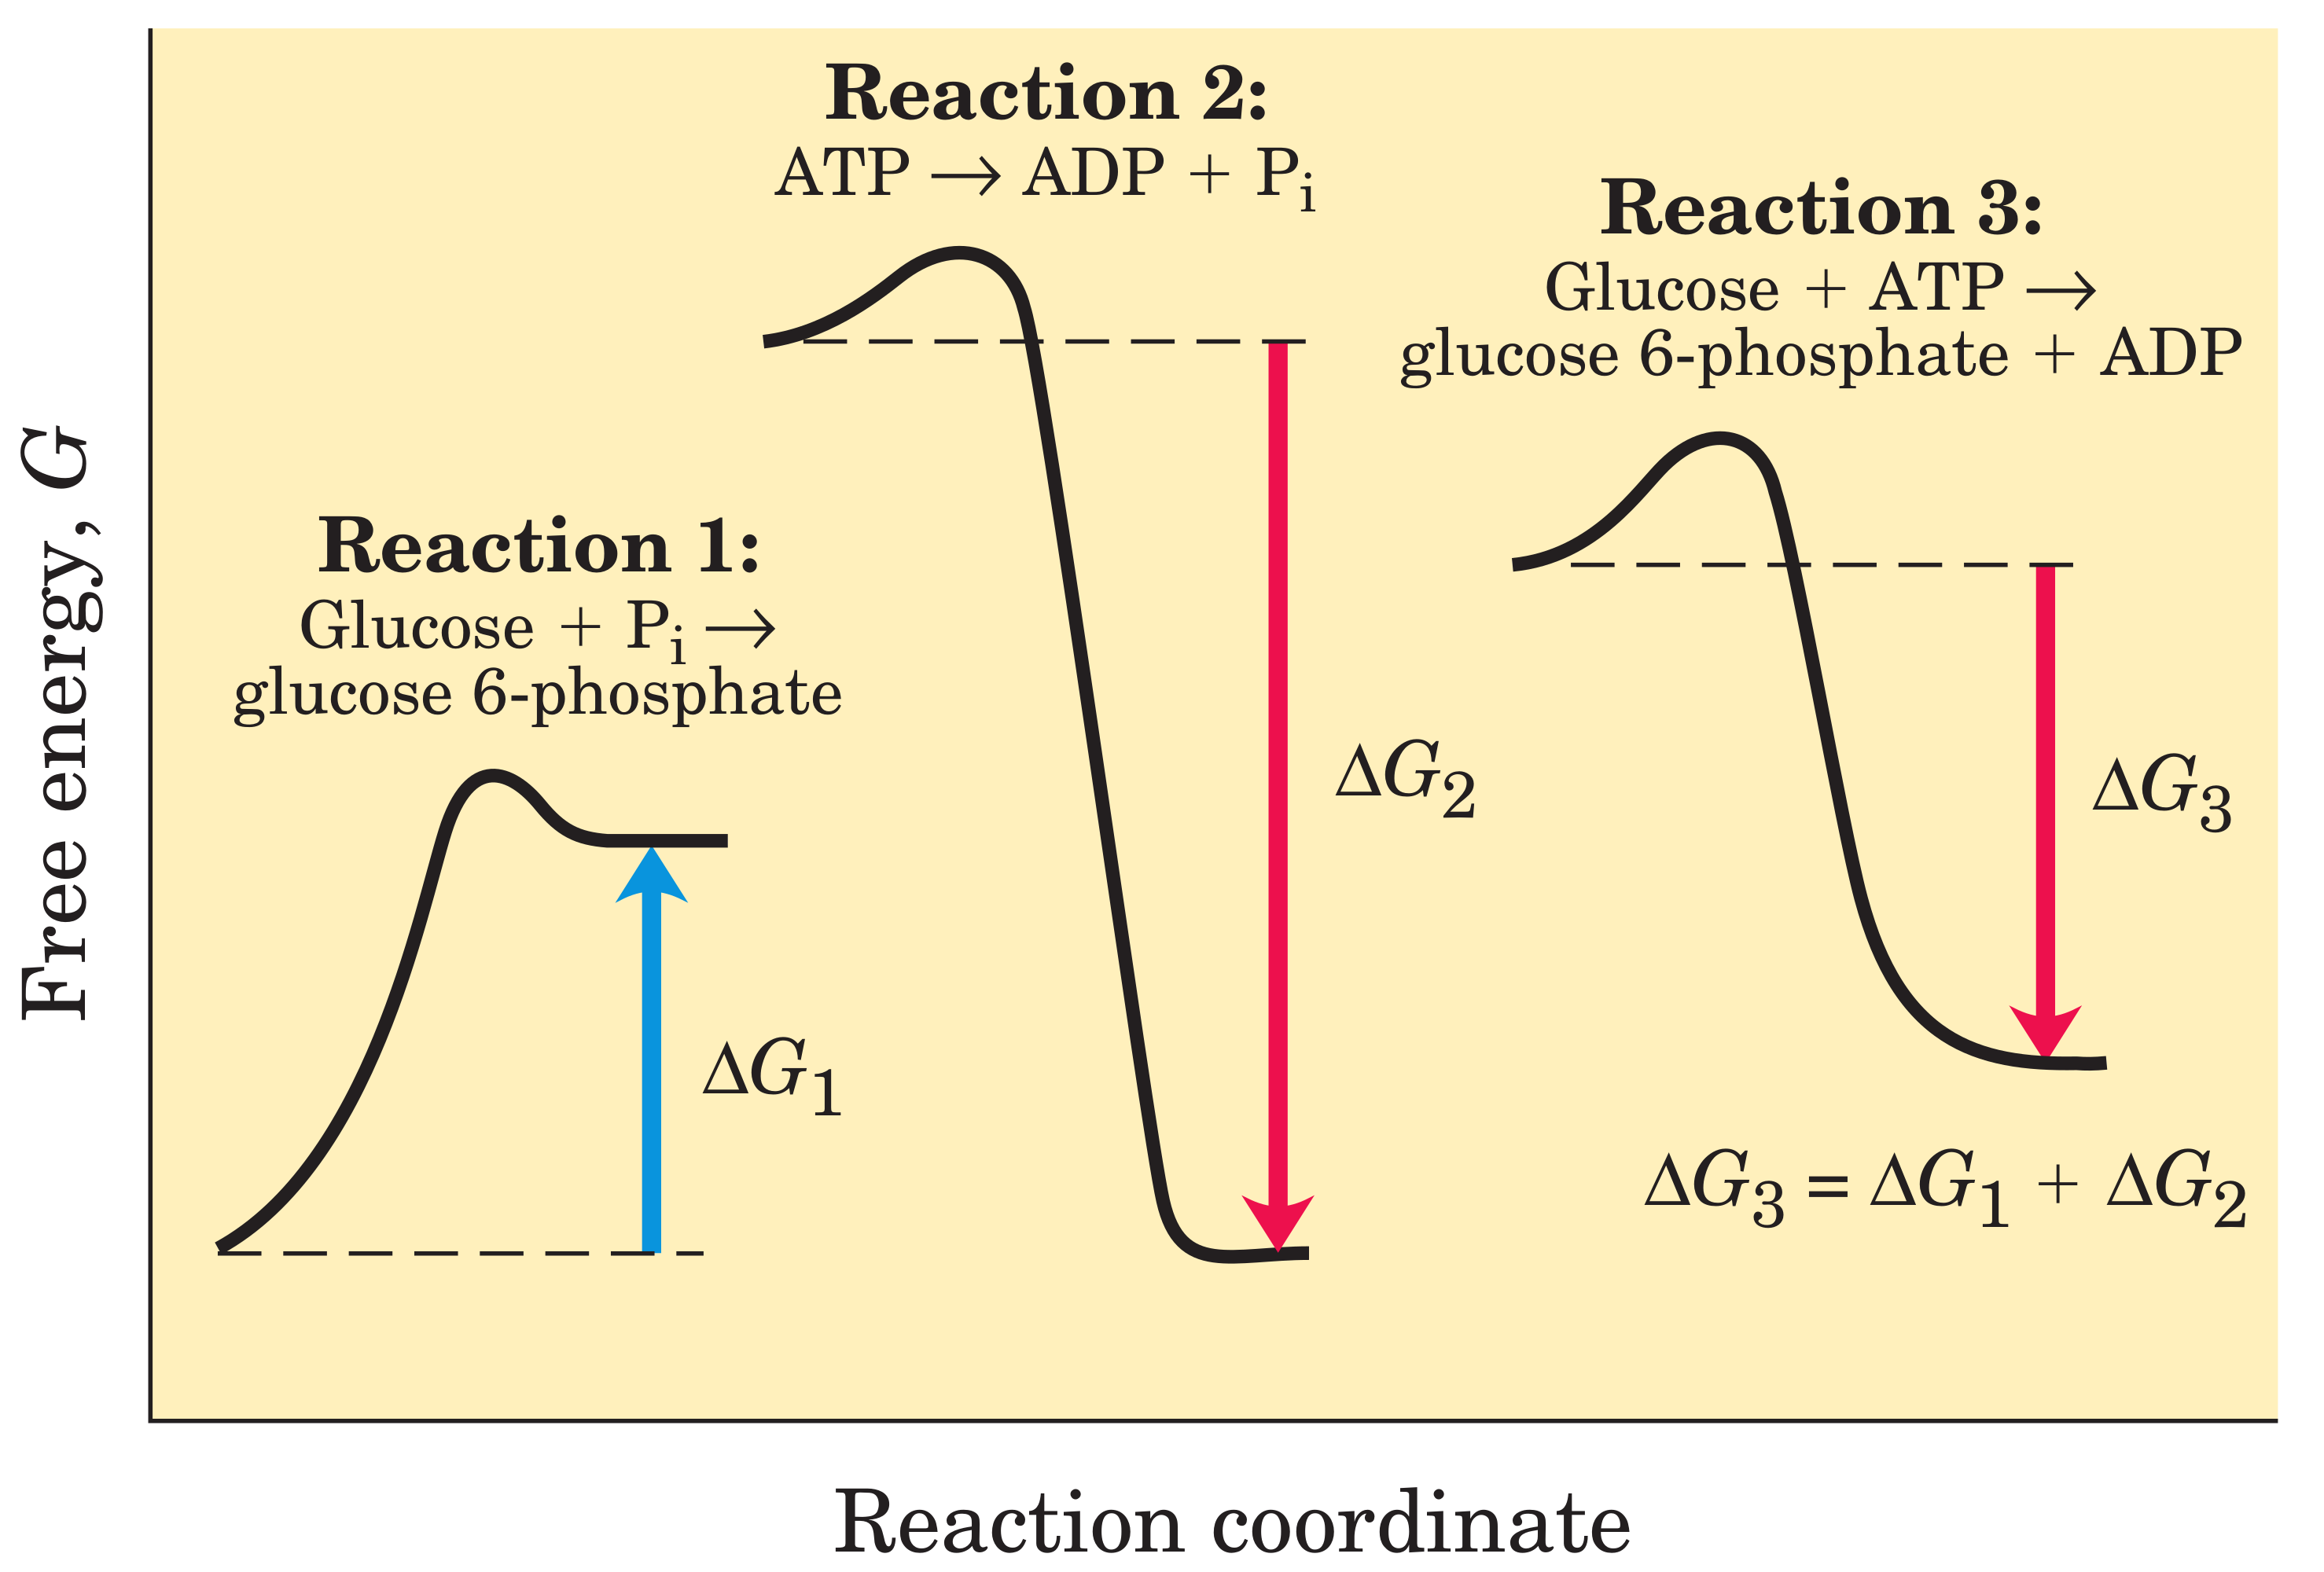
\includegraphics[width=0.6\linewidth]{freeEchangeFig.png}
		\caption{Free Energy landscapes of three reactions, showing the different flux-constraints imposed in our model. Figure reproduced from \cite{principlesofbio}}
		\label{fig:freeEchangeFig}
	\end{figure}

	The constraints imposed on the flux of each reaction, depending on the free energy change of them are as follows: for the $m$th reaction the flux $v_m$ has to satisfy $0\leq v_m \leq 1 $ if $\Delta G \leq -L$~eV, $-1\leq v_m \leq 0 $ if $\Delta G \geq L$~eV. As in the real world the reactions happening in a cell are usually reversible.  An example for this is is the reaction of carbonic acid and water H$_2$CO$_3$$_{(l)}$ + H$_2$O$_{(l)} \leftrightarrows$ HCO$^-_3$$_{(aq)}$+H$_3$O$^+$$_{(aq)}$. We allow reactions with free energy change between a constant $-L$ and $L$ eV to happen in any direction. Currently the value of $L=10$~eV but it is a parameter easily changed in the program. In Figure~\ref{fig:freeEchangeFig} we show possible cases of this. Assuming $\Delta G_1 > L$ Reaction 1 would have it's flux restricted as $-1\leq v_1 \leq 0$, also if $\Delta G_2 < -L$ $v_2$ is restricted as $0 \leq v_2 \leq 1$, and if $|\Delta G_3 | \leq L$ we have $-0.5 \leq v_3 \leq 0.5$. 

	In real life the likelihood of these reactions happening, and so the flux through them depends on the height of the potential barrier between the original substrates and the end products. If the barrier is high the reaction might not happen unless the amount of energy required to overcome it is invested. Cells are able to lower the heights of such barriers using catalytic enzymes, therefore our model is not unrealistic by neglecting their role in determining the directions and fluxes of the reactions. 

\subsection{In silico Evolution}
\label{sub:implementing evolution}
To simulate biological evolution on a computer we need three things: replication, mutation and competition. The sophisticated interplay of random mutations and the more deterministic selection gives rise to the success of evolution. The basics of these concepts can easily be implemented in our program, giving a process similar to biological evolution. Our simulations always start with a homogeneous population, all cells are identical. The population later diverges as a result of random mutations. The real evolution of the genomes of organisms uses a variety of methods some of which are discussed in Section \ref{chap:evolution}. Of these, our cells use point mutations and later horizontal gene transfer.
	
	Point mutations either add or delete a reaction to the MN. Simply adding a reaction to those available to the cell at random from the list of all the reactions is unlikely to result in a reaction that could be used by the cell. This is because with a high probability the added reaction would be disconnected from the current MN. As discussed in Section \ref{sub:Flux Balance analysis} the flux through these reactions would be zero. Therefore when adding reactions, we only consider those that are linked  to one of the current reactions, either by using a compound that  the network is capable of producing, or providing one that it can consume. EXAMPLE FOR TRIAL NETWORK USED IN FBA SECTION? This way the graph of the reactions and compounds available to the cell stays a connected graph (disregarding deletions). Choosing the list of reactions that can be added uses the neighbour-list defined in OUR ALGORITHM APPENDIX X. When deleting a reaction every currently available reaction has equal probability of being deleted. This can and does result in disconnected graphs, but such disconnected parts are usually small, otherwise they bear too high a cost to maintain and are therefore an evolutionary disadvantage.
	
The most elementary event in a population of our organisms is a reproduction, implemented using the Moran process \cite{moranprocess} 

At every step of the Moran process a single member of the population is chosen to reproduce (with or without mutations) and an other member of the population dies, to keep the size of the population constant. At every such step the cell has some probability of mutating, both for a point mutation ($P_{point}$), and for horizontal gene transfer ($P_{HGT}$) from an other randomly chosen cell.  This process is a random walk in the space of all possible genes or MN-s allowed by the chemistry of the cells  This walk is then mapped to the fitness landscape using the goal function of the cells.

There are two contributions to the fitness measure of a cell, it's energy production, and the number of reactions in it's MN.  In the original goal function a fitness score of $1$ is awarded for every ADP $\rightarrow$ ATP executed by the cell. For every reaction in the MN the cell pays a small cost $k_{reac}$  from the fitness score of the cell. This is because cells usually control their reactions through the use of enzymes that they have to manufacture, and code in their genetic code. Should we not include this cost the cell's MN-s could grow without bounds until every reaction in our list would appear within them. This could then be considered a best network. Later we consider more complex goal functions that reward biomass production, at different weights compared to the energy production. 

The probability density function (PDF) of which cell is selected for reproduction is proportional to the fitness of each cell (with the CAVEAT that cells with negative fitness are deemed unviable and are not allowed to reproduce). To know this PDF it is necessary to know the fitness of each cell at any given time point (for the normalization), and therefore it would be impractical to use this to chose the cell that will reproduce. Instead we sample as follows: 
\begin{enumerate}
	\item We uniformly chose a cell in our population --- $c_i$
	\item We generate a random number from the distribution $U \left( r,M \right)$ where $M$ is the maximal fitness value a cell can take
	\item If the fitness of $c_i$,  $F_{c_i} \geq r$ we accept the change, if not we start the process again
\end{enumerate}

This process can be shown to result in a sampling of cells equivalent to that of the PDF proportional to the fitness of each cell.

DETAILED BALANCE ~ GIBBS etc probs not

\subsection{Flux Balance analysis}
\label{sub:Flux Balance analysis}

\textbf{Detailed description $\rightarrow$ equations, example matrix? Which fluxes are free? Which fluxes are limited? GLPK }



	To calculate the throughput of the metabolic network of our organisms we use flux balance analysis \cite{whatisfluxbalance}. 	

	The goal of flux balance analysis is to calculate the steady state fluxes ($\mathbf{v}$) through all the reactions, subject to some constraints, (described later in this section), while maximizing a linear function $Z=\mathbf{c}^T \mathbf{v}$ of the fluxes (called goal function) in the solution space allowed by the constraints. 

	\begin{figure}[htpb]
		\centering
		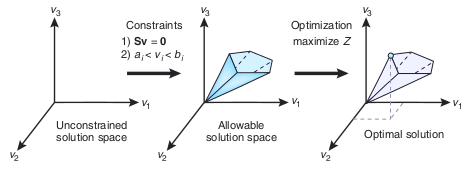
\includegraphics[width=0.8\linewidth]{fba_frompaper.png}
		\caption{The process of flux balance analysis. First we apply the steady state constraints along with FURTHER CONSTRAINTS on the fluxes, then we maximize the goal function in the allowable solution space found. Figure reproduced from \cite[]{whatisfluxbalance} }
		\label{fig:fluxbalance}
	\end{figure}

	When using flux balance analysis we represent the MN as a stoichiometric matrix $S$ ($m\times n$), with each row corresponding to a compound in the network ($n$ compounds), and each column corresponding to a reaction ($m$ reactions). In each column we have the stoichiometric coefficients of the given reaction that correspond to the compound of the given row. Negative stoichiometric coefficients are used for the metabolites consumed, positive for those produced, and zeros for the metabolites that do not participate in the given reaction.
	
	We want to find a set of fluxes  $\mathbf{v}=\left( v_1,v_2,...,v_m \right)$ that are steady state fluxes, satisfying $S\mathbf{v}=\mathbf{0}$ (the allowable solution space in Figure~\ref{fig:fluxbalance}). These equations take the form
	
	\begin{equation}\label{eq:steadystateeq}
		\begin{matrix}
			S_{1,1} v_1 + S_{1,2} v_2 + ... + S_{1,m} v_m=0 \\
			S_{2,1} v_1 + S_{2,2} v_2 + ... + S_{2,m} v_m=0 \\
			... \\
			S_{n,1} v_1 + S_{n,2} v_2 + ... + S_{n,m} v_m=0 \\
		\end{matrix}
	\end{equation}
	The steady state assumption of the method means that the amount of any given compound produced in the reactions should equal the amount consumed by other reactions, except for some special compounds. These special compounds are considered the nutrients and the end-products of the MN. For example the nutrients of our network on Figure~\ref {fig:examplenetwork} is FIRST COMPOUND, water and $O_2$, while it's end products are pyruvate and $CO_2$. Incorporating compounds that the MN can import/export to it's environment to flux balance analysis could be done through relaxing the constraint that the equation corresponding to the given compound among those in Equation \ref{eq:steadystateeq} have to equal zero. This introduces complications, as often the amount of these compounds produced appears in the goal function  $Z=\mathbf{c}^T \mathbf{v}$. To overcome this we introduce auxiliary reactions to the stoichiometric matrix $S$, for the compounds the cell consumes and produces. Such an auxiliary reaction is for example " $ \rightarrow H_2O$", that "creates water out of nothing", or in other words corresponds to the potential water intake of the cell ENABLING THE CELL TO TAKE UP WATER?


	In the allowable solution space we want to maximize the goal function $Z \left( \mathbf{v} \right)$ The form of the goal function is $Z=\mathbf{c}^T \mathbf{v}$ with the elements of $\mathbf{c}$ being the weights of the fluxes of each reaction in the goal function. In the simplest cases $c_i=0$ for all but a single value of $i$, in which case the goal is to maximize the flux through a single reaction, which is often chosen to be the biomass removing auxiliary equation. In our case the original goal function used is the one converting ATP to ADP. This reaction occurs in cells, (ATP~+H$_2$O~$\rightarrow$~ADP~+~P$_i$), and it releases energy. As cells store energy in ATP molecules,  by maximizing the flux through the ATP producing reaction, we are maximizing the energy output of the cell. In many cases this is synonymous with maximizing the growth rate of the cell. (CITATION). OTHER GOAL FUNCTIONS?
	
	There are many software packages capable of solving linear programming problems, we use the Gnu Linear Programming Kit (GLPK) \cite{glpk}. GLPK is implemented in C, and has all the functionality we need to calculate the fitness of our metabolic network. For the code calculating the fitnesses see the function calcThroughput in APPENDIX.


\subsection{Example of flux balance analysis}
\label{sub:example_of_flux_balance_analysis}

Here we give an example of how flux balance analysis is calculated. We consider a toy network, that has an easily verifiable solution. The network is shown on Figure~\ref{fig:examplenetwork}, and it is one this part of the program was tested when written. For the purpose of this example let us consider the cost of a reaction is $k_{reac}=0.01$.


	The metabolites of the network (in green) have been denoted by letters A, B and D for brevity. The stoichiometric matrix of this metabolic network is shown at Equation~\ref{eq:examplematrix} (below), with the metabolites the rows correspond to are shown on the left of the matrix. The first three columns of the matrix correspond to reactions $5151$, $5133$ and $131$ respectively. The other columns correspond to auxiliary reactions, providing the nutrient of the network (A), removing the end-product (lactate), providing water, providing CO$_2$, and converting ATP to ADP in this order.

\begin{figure}[htbp]
	\centering
	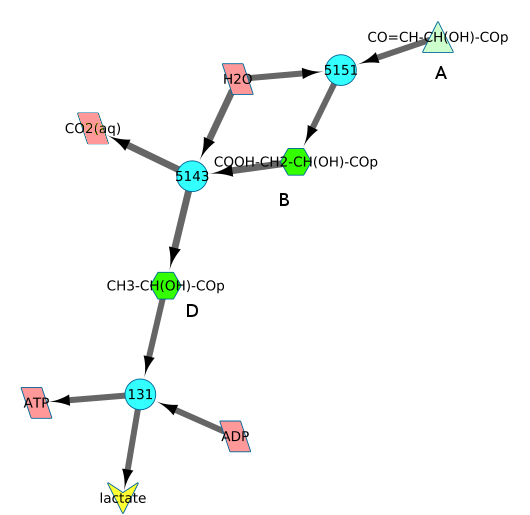
\includegraphics[width=0.5\linewidth]{initial_network_ABC.png}
	\caption{Example of a simple network. Reactions: light blue, metabolites: green, nutrient: light green, end-product: yellow, internal metabolites:red}
	\label{fig:examplenetwork}
\end{figure}

	\begin{equation}
	\begin{matrix}
		\texttt{A}   \\
		\texttt{B}\\
		\texttt{D}\\
		\texttt{lactate}\\
		\texttt{water}\\
		\texttt{CO}_2\\
		\texttt{ATP}\\
		\texttt{ADP}
	\end{matrix}
	,S=
	\begin{pmatrix}
			%\hline Fluxes: & 1 & 1 & 1 & 1 & 1 & 3 & -3 & \color{red} $\mathbf{1}$ \\
			%\hline	Reaction: & 5151& 5143 & 131 & \multicolumn{4}{c|}{Auxiliary }& Target \\
			  -1 &  0 &  0 & +1 &  0 &  0 & 0 & 0 & \\ 
			  +1 & -1 &  0 &  0 &  0 &  0 & 0 &0 &  \\ 
			  0 & +1 & -1 &  0 &  0 &  0 & 0 & 0 & \\ 
			  0  &  0 & +1 &  0 & -1 &  0 & 0 & 0 & \\ 
			  -1 & -1 &  0 &  0 &  0 &+1  & 0 & 0 & \\ 
			  +1 & +1 &  0 &  0 &  0 &  0 & -1&0 &  \\ 
			  0 & +1 &  0 &  0 &  0 & 0 &0 & -1 &\\ 
			  0 & -1 &  0 &  0 &  0 & 0 &0 & +1 & \\ 
			  
		\end{pmatrix} 
		\label{eq:examplematrix}
	\end{equation}


	The linear equations that are implied by $S\mathbf{v}=\mathbf{0}$ for the example network of Figure~\ref{fig:examplenetwork} are shown below, at Equation \ref{eq:lineqs}. Constraints on the system are imposed in two ways. Firstly by $S\mathbf{v}=0$ we require that the fluxes represent the steady state solution, and secondly by restricting the values of $v_i$ by inequalities ($v_{lower,i}\leq v_i \leq v_{higher,i}$) we can restrict the flux of individual reactions, their directions, and the amount of COMPOUNDS the cell can take up and dispose of. 
	

	\begin{equation}\label{eq:lineqs}
	\begin{matrix}
		\texttt{A}   \\
		\texttt{B}\\
		\texttt{D}\\
		\texttt{lactate}\\
		\texttt{water}\\
		\texttt{CO}_2\\
		\texttt{ATP}\\
		\texttt{ADP}
	\end{matrix}
		\begin{matrix}
			- v_1+v_4=0 \\
			v_1-v_2=0 \\
			v_2-v_3=0 \\
			v_3-v_5=0 \\
			-v_1-v_2+v_6=0 \\
			v_1+v_2-v_7=0 \\
			v_2-v_8=0 \\
			-v_2+v_8=0
		\end{matrix}
	\end{equation}

	The bounds on the given reactions are as follows: 

	\begin{equation}\label{eq:bounds}
		\begin{matrix}
			0\leq v_1 \leq 1\\
			0\leq v_2 \leq 1\\
			0\leq v_3 \leq 1\\
			0\leq v_4 \leq 10\\
			0\leq v_5 \leq \infty \\
			0\leq v_6 \leq 40\\
			0\leq v_7 \leq 40\\
			0\leq v_8 \leq \infty\\
		\end{matrix}
	\end{equation}

	The limiting fluxes should in any case be those of the real reactions (in our case $v_1, v_2,$ and $v_3$. The cell's nutrient intake ($v_4$) is set to a high but finite value, this is important as a this puts a high bound on the fitness function. Such a theoretical upper bound for the fitness function must be known, as it is used in the algorithm when we select the next cell that reproduces. The cell's water intake and CO$_2$ disposal are limited by a high value for the same reason. Care is taken in order to keep these values high enough not to be limiting for the evolution of the network. REPHRASE The pyruvate removal and the ATP $\rightarrow$ ADP conversion reactions need not be bounded, as they are limited by the nutrient uptake of the cell. 

	The goal function in this case is $v_8$, the energy output of the cell, this is to be maximized within the constraints.

	The optimal solution of the equations with the bounds given at Equation \ref{eq:bounds} is 
	\begin{equation}\label{eq:solution}
		v_1=1 , v_2=1, v_3=1, v_4=1, v_5=1, v_6=2, v_7=2, v_8=1
	\end{equation}
	Giving the value of the goal function to be $Z=v_8=1$. As the MN has $3$ reactions the final fitness value for it would be $Z-3\times k_{reac}=1-3\times 0.01=0.97$
\subsection{Data analysis}
\label{sub:visualization}

To visualize the resulting MN-s we use the open source biological network visualization tool Cytoscape \cite{cytoscape}. Figures showing metabolic networks in this work have been generated using this software (eg.  Figure~\ref{fig:examplenetwork}) for brevity. Our program was equipped with the functionality to export MN-s into the \texttt{XGMML} format that Cytoscape can read in. 

While MN-s can be visually compared using Cytoscape, doing so for more than a handful of networks is a cumbersome task, therefore we considered some summary statistics to compare MN-s resulting from our simulations.

While the simulation is running, every few thousand generations some key descriptors of the populations are written out to a log file. This allows us to monitor the evolution of the populations while the simulation is running, and also to plot the timeline of their evolution. Examples of such graphs can be found in Section \ref{sec:results} (eg. Figure~\ref{fig:simulation1} ). These descriptors are: the fitness of the fittest network in the population, the average fitness of the population, the entropy of the population, the number of reactions in the fittest network, the average number of reactions in the population the number of used reactions (those with non-zero flux) in the best MN, and the average number of such reactions per MN in the population. 


Entropy is used as one of the measures of the diversity of the population. It is calculated as: $S=- \sum^{M}_{i=1} n_i \log n_i $ where $n_i$ denotes the number of cells of type $i$, and the sum runs through all the different types of cells in the population.  As we are considering a population with $N=100$ cells, the minimal entropy is $S_{min}=-100\log100=-460.52$, this value is attained when every cell in the population is identical ($p_{i_1}=100$, and $p_i=0$ for other $i$ values), as is the case initially in our populations. It's maximal value is $S_{max}=0$ attained when every cell is different in the population. This happens when the mutation rate is very high (eg. $P_{point}=1$). 


To compare networks between populations we define a similarity index $M_{i,j}$ between two MN-s $i$ and $j$, calculated as follows: we count the reactions appearing in both MN-s, then divide this count by the number of reactions in the larger network. $0\leq M_{i,j} \leq 1$, with these extreme values attained if the two MN-s share no reactions, and if they are identical, respectively. We calculate two similarity indices for each pair of MN-s, one for every reaction in the two MN-s ($M_{i,j,all}$) and one only for those reactions that have non-zero flux through them in the optimal solution ($M_{i,j,used}$). This is an important distinction, as for a high mutation rate, and small $k_{reac}$ value the two MN-s might have a lot of unused reactions that differ amongst them, but their used reactions could be the same.  As the indices are symmetric ($M_{i,j,all}=M_{j,i,all}$ and  $M_{i,j,used}=M_{j,i,used}$) instead of two separate plots, we plot 

$$
M_{i,j}= \left\{
	\begin{array}{ll}
		M_{i,j,all} & \quad i \leq j \\
		M_{i,j,used} & \quad \text{otherwise}
	\end{array}
\right.
$$

Thus we show the similarity indices calculated using all reactions above the diagonal of the plot, and those calculated using the used reactions below the diagonal. The diagonal entries are always $1$-s as any network is equivalent to itself. We plot the two regions separated to make distinguishing between the two parts easy.

While the simulations are running, we save the states of the populations at 10 occasions, both to be used as checkpoints if the calculation doesn't finish, and also to be able to look at how the networks evolved. At these checkpoints the MN of every cell in the population are written out (in the \texttt{XGMML} format). This allows both the visualization of the networks and also their comparison using the similarity indices between them. As plotting the similarity indices as a matrix (as in FIGURE EXAMPLE) for every population at every checkpoint would be unpractical, we instead consider the similarity indices of MN-s within a population compared to the fittest network in the population, resulting in a vector of $N-1$ similarity indices (we don't compare the fittest network with itself). This would correspond to the first column (or row) of each population on the similarity matrix plot, for example Figure~\ref{fig:simmatrix_firstjob}.

These similarity indices are then summarized using the Inverse Participation Ratio of them. EXPLAIN  The similarity indices of each population are divided into 10 bins, and the IPR of the proportion of elements in the bin are calculated, using $IPR= \sum^{10}_{i=1} \frac{1}{p_i^2} $ where $p_i$ is the proportion of similarity indices in bin $i$ (this ensures normalization, $ \sum^{10}_{i=1} p_i=1$). The minimum of this IPR value is $1$, attained for a completely homogeneous population, while the maximum of $10$ is attained when each of the 10 bins have an equal amount of similarity indices within them (the most disordered state).  At each checkpoint the IPR of the two similarity indices $M_{i,j,all}$ and $M_{i,j,used}$ are calculated along with the IPR of the fitness values at the checkpoint. 

\textbf{IPR: How to calculate, why is it useful? Can be calculated for nonzero flux reactions or all available ones too. IPR vs Entropy}






\subsection{Technical bits RENAME}
\label{sub:technical_bits}

(In a population usually there are multiple "copies" of any given cell, as the rate of mutations is low, eg. for $p_{point}=0.1$ only every tenth reproduction results in a new type of cell.)

	Whenever we add a reaction to a MN we have to find the reactions that connect to the current network, through at least one shared metabolite, as described in section \ref{sub:implementing evolution}. It is very time consuming to list all metabolites currently in the network, then search through all the reactions to see if any of the used metabolites are used within them. To remedy this at the beginning of the program a neighbour-list is generated that contains for every reaction a list of neighbouring reactions, that share at least 1 compound with it (excluding internal metabolites). For example in our example network on Figure~\ref{fig:examplenetwork} reactions 131 and 5143 are neighbouring, as they share the metabolite CH$_3$-CH(OH)-COP, but reactions 131 and 5151 are not neighbouring. Using this neighbour-list our program can now rapidly find the possible reactions to add to a network. 

	An important component of a Monte Carlo simulation is the source of pseudorandom numbers. In our program we use the Mersenne Twister \cite{mersennetwister} generator, provided by the boost C++ libraries \cite{boostlibraries}. This generator is fast, provides high-quality pseudorandom numbers and has a period of $2^{19937}-1$, and will therefore provide more than enough pseudorandom numbers for our simulations.

	To speed up calculations we performed multiple parallel simulations of populations on different computers. In order for every population to be different, we used different initial values to seed the pseudorandom number generator. For the sake of reproducibility these seeds are noted with the output of the simulations. 


\section{Results}
\label{sec:results}

\textbf{Initial simulations, 100\% mutation rate, very diverse populations}

\subsection{Test simulation}
\label{sub:test_simulation}

\begin{figure}[htpb]
	\centering
	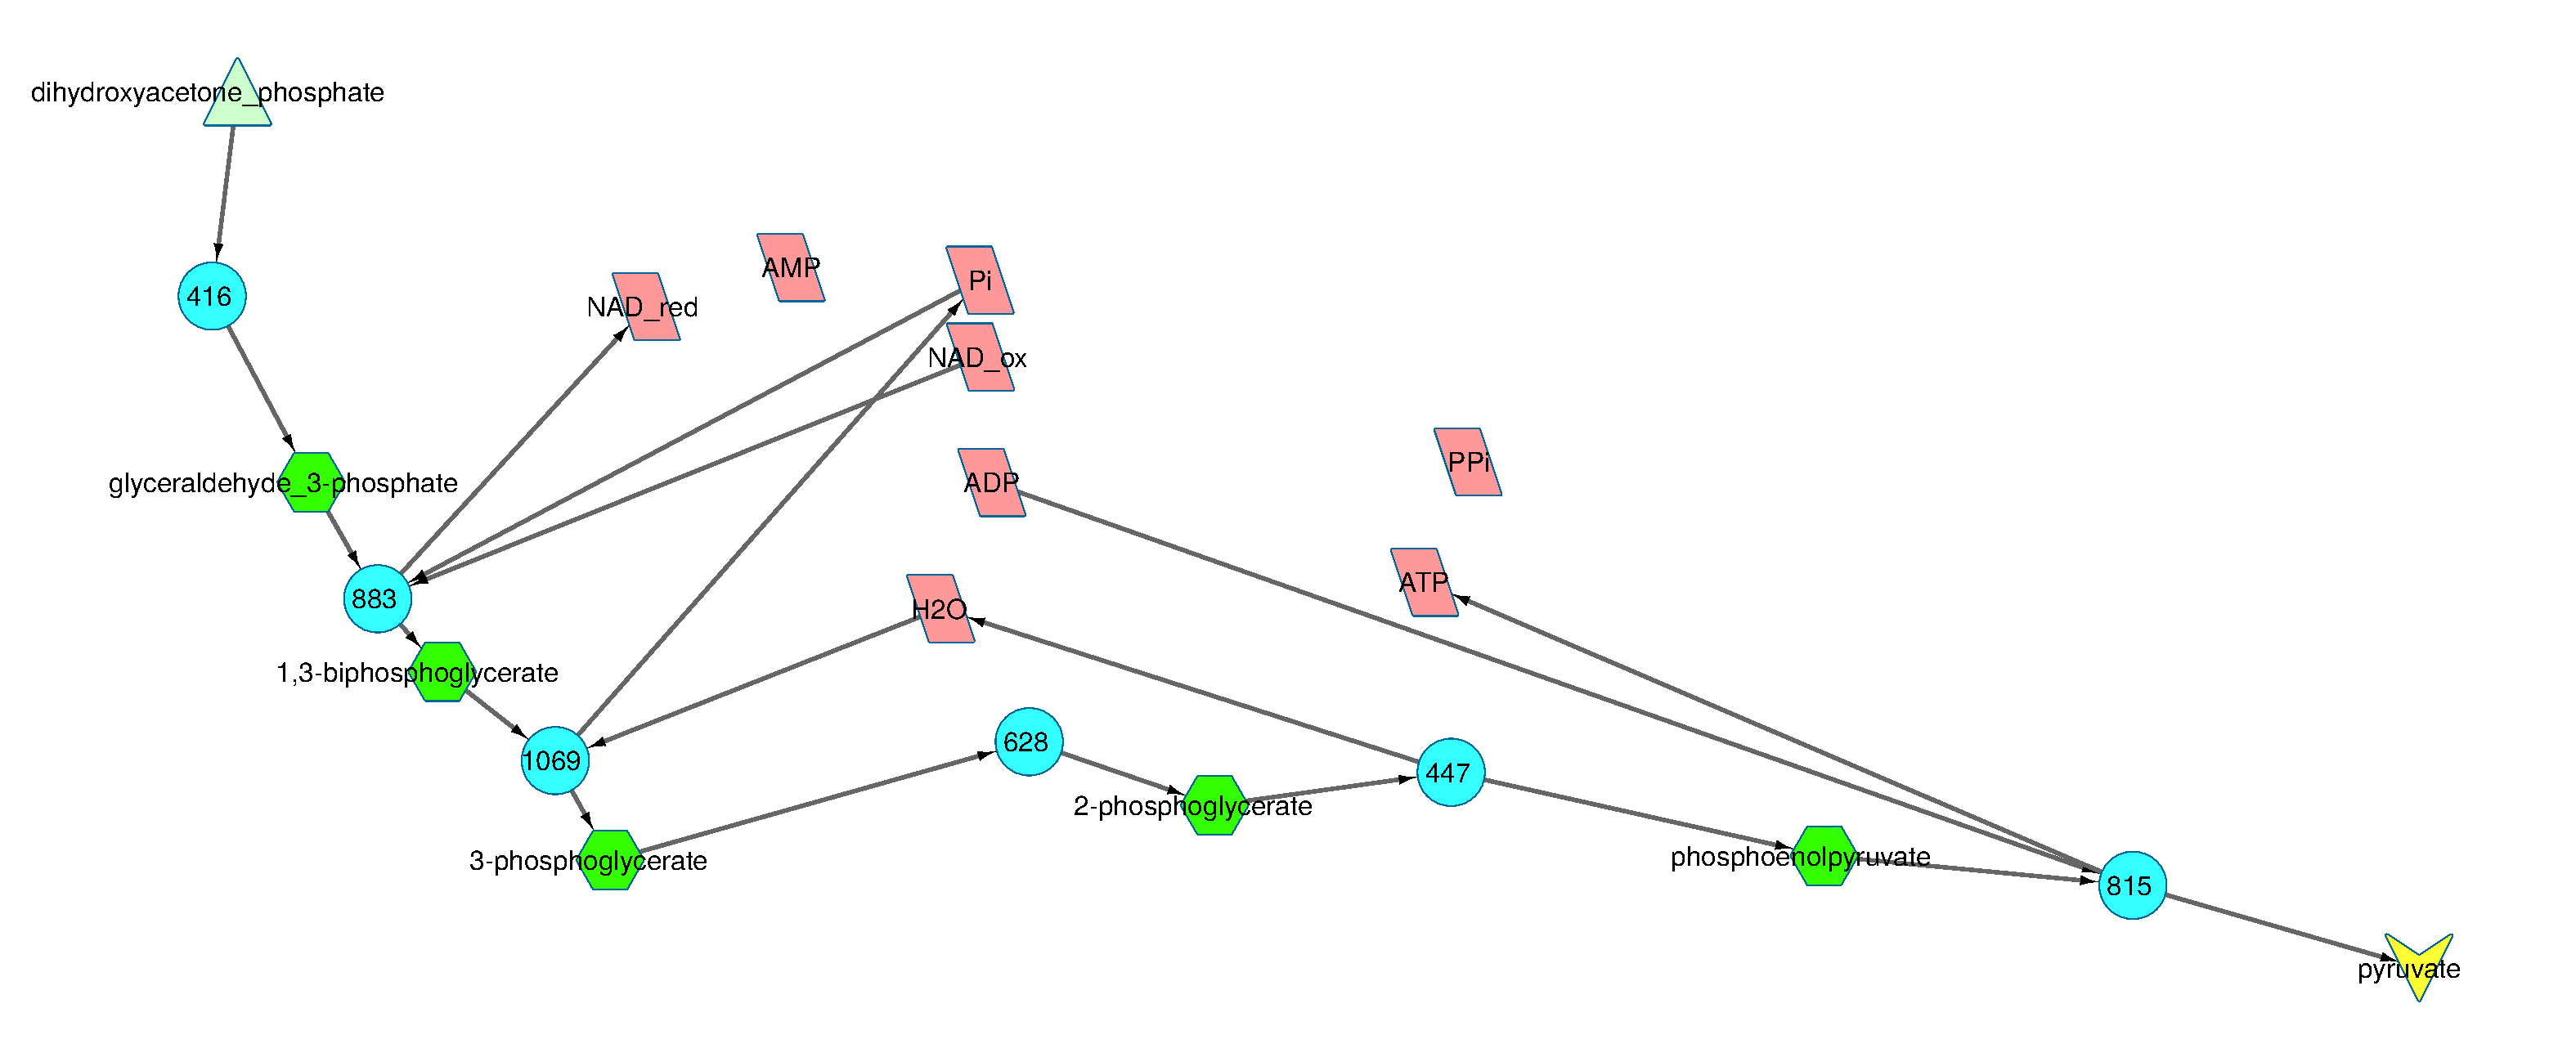
\includegraphics[width=1\linewidth]{trunk_glyc_init.pdf}
	\caption{Trunk of the glycolytic pathway plus few reactions at the beginning LARGER TEXT}
	\label{fig:truncglycinit}
\end{figure}

The first simulation we run used a modified version of the trunk of glycolysis as a starting network. This modified network starts from Dihydoxyacetone phosphate (DHAP), one of the products of the upper part of glycolysis,  and ends in Pyruvate. The starting network is shown on Figure~\ref{fig:truncglycinit}.  Reaction $416$ was added to the usual lower glycolytic pathway at the beginning of the MN, this reaction transforms DHAP into G3P the compound normally considered the first metabolite of lower glycolysis.  Apart from this the ATP producing reaction $633$ was removed, in exchange for $1069$, that fulfills a similar role to $663$, but instead of creating ATP from ADP it discards the phosphate group it SHEDS from 1,3 biphosphorglycerate.

The initial ATP flux of this network is $0.5$, with the limiting reaction being $883$, that has a free energy change of $1.71$ eV at the conditions given by Table \ref{environmentTable}. This is a good initial network as it has plenty of potential to improve, eg by "rediscovering" reaction $633$, or finding completely new paths from the nutrient of the MN to the end product. For the sake of brevity we shall refer to this simulation as Simulation $1$.

The fitness cost of having a reaction within the MN was set to $k_{reac}=0.001$ with the rate of point mutations as $P_{point}=1$ in order to have as much change and improvements as possible. The fitness function used here was the flux of ADP to ATP conversion minus $k_{reac}$ times the number of reactions in the MN.

When running the simulations, we started with 20 identical, uniform populations with $100$ cells each, and provided a different seed for the pseudorandom-number generators used, therefore the populations evolved independently from one another. Not all the 20 populations finish the simulation due to technical difficulties. Of those that did, we generally show diagnostic plots for 3 typical populations that showed some improvement during the simulation.




\begin{figure}[htpb]
	\centering
	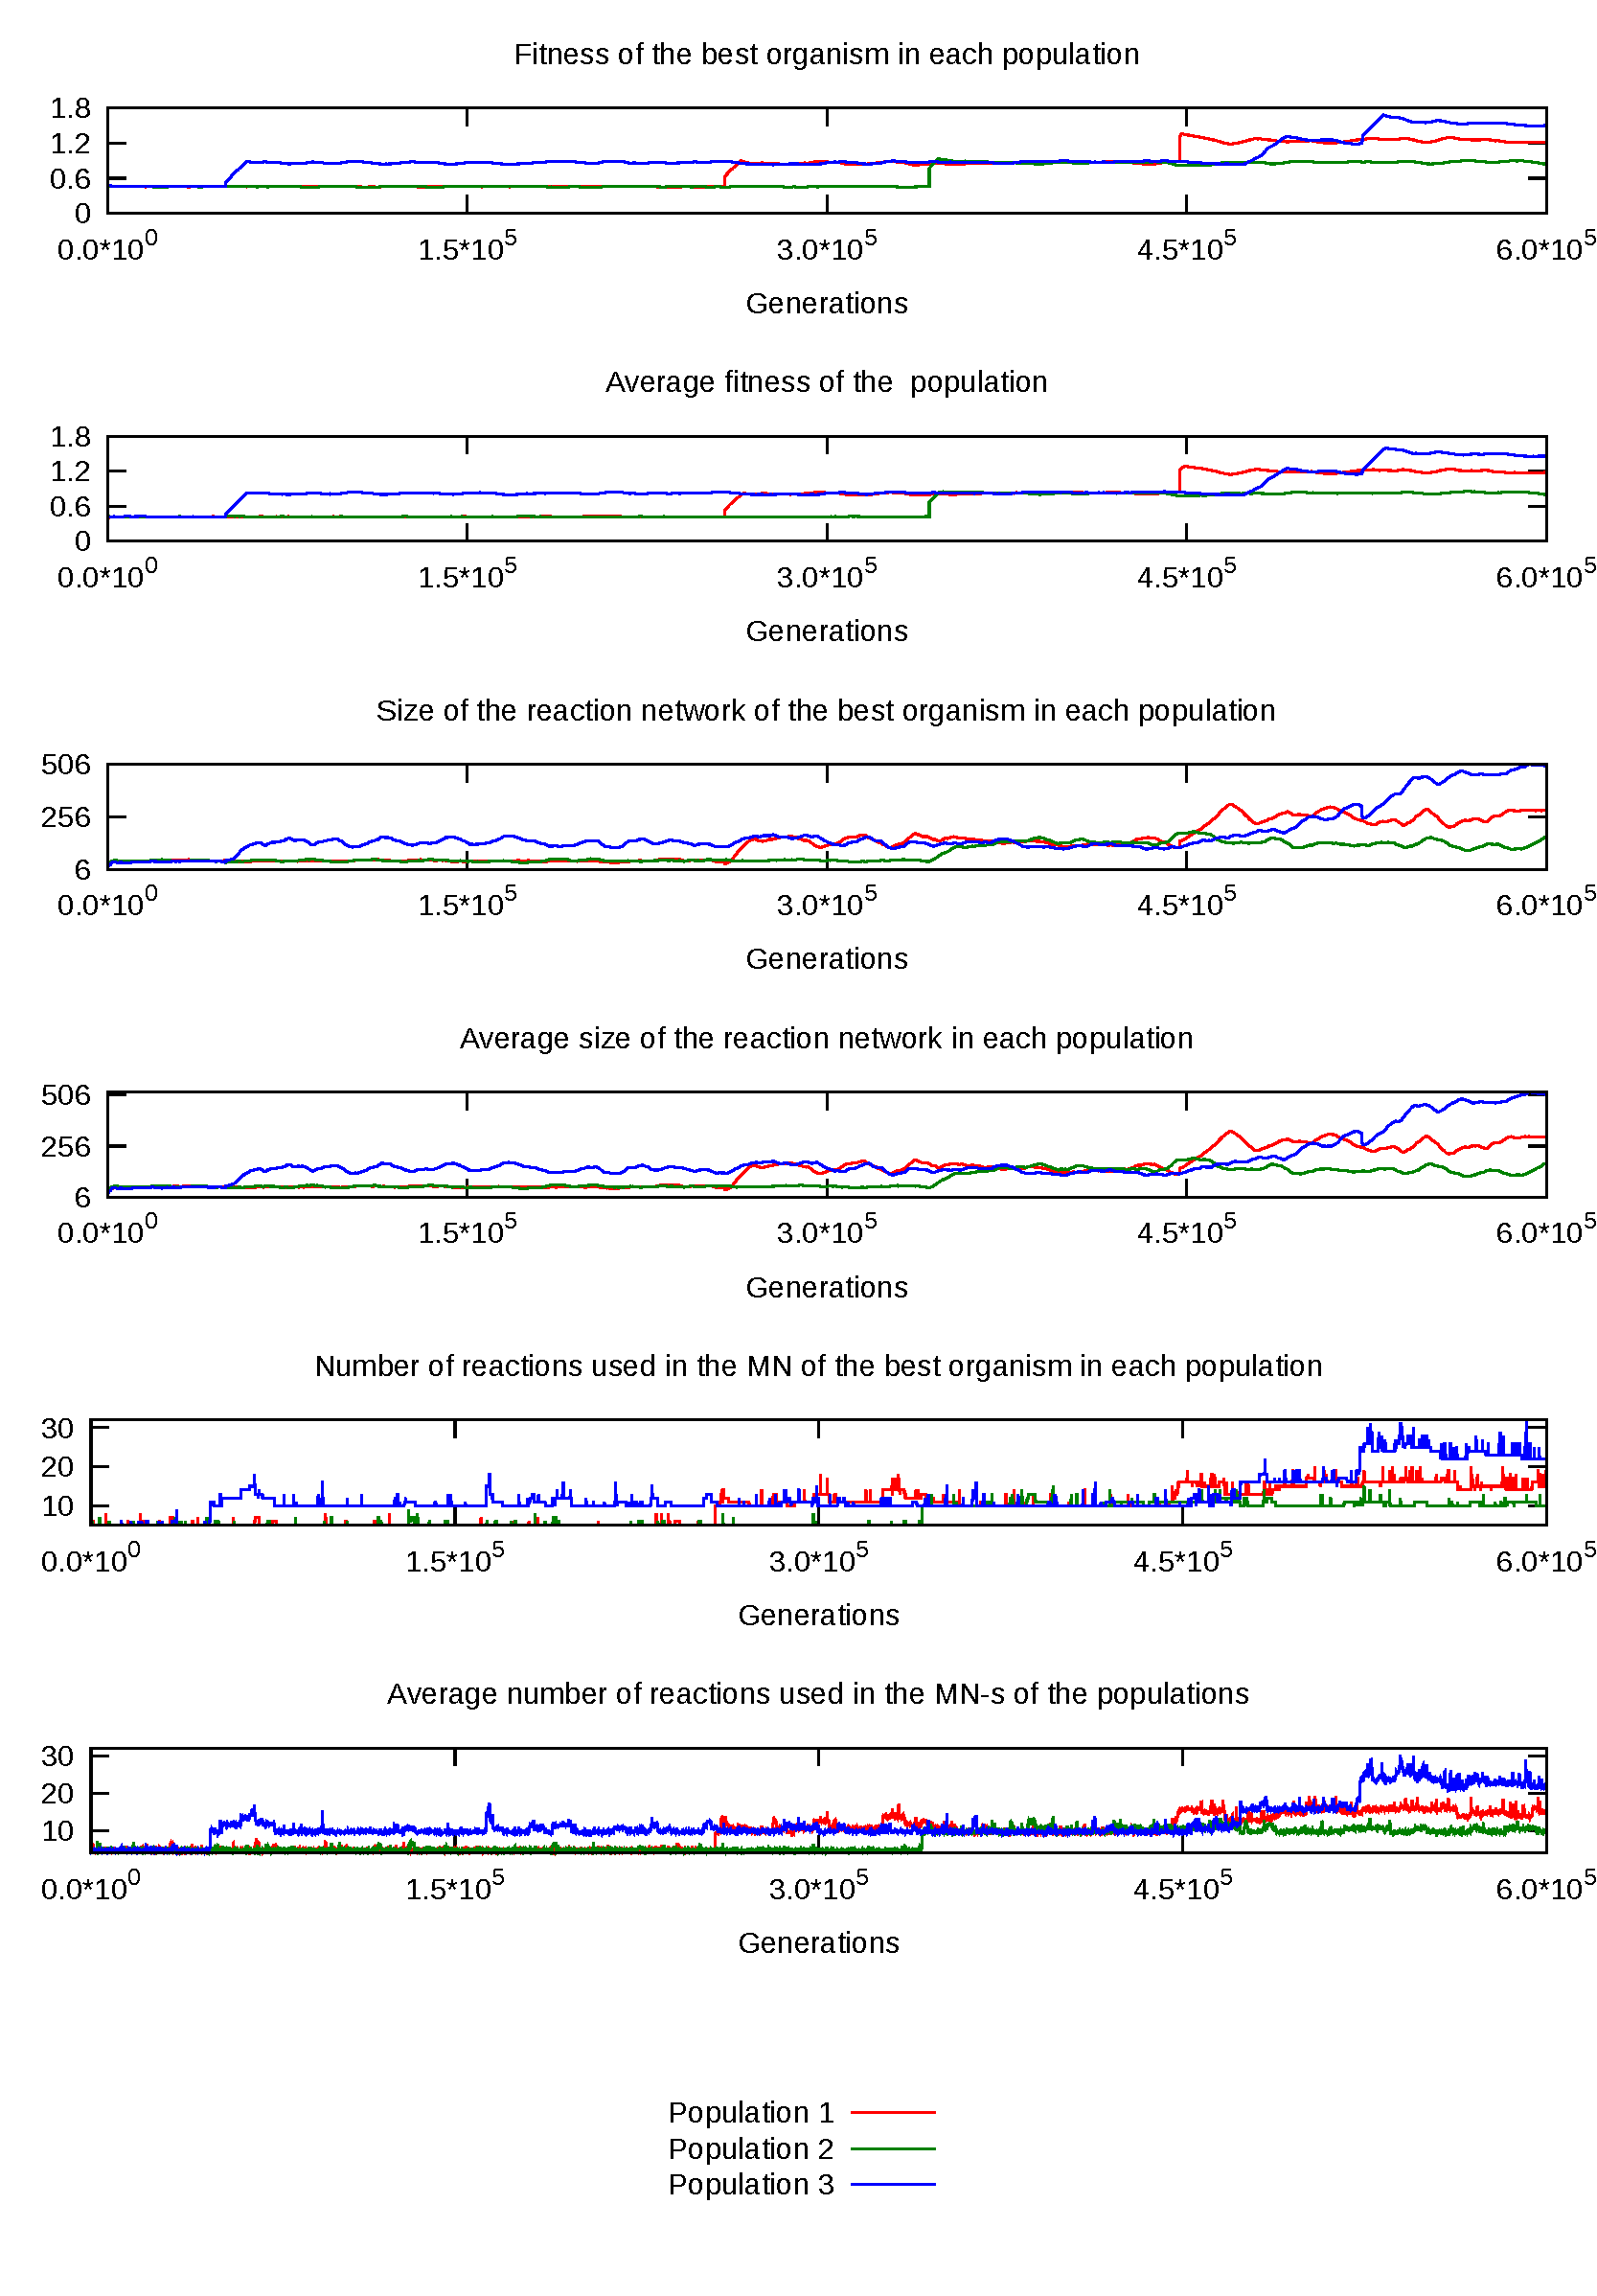
\includegraphics[width=1\linewidth]{simulation1.pdf}
	\caption{Diagnostic plots for 3 typical populations of Simulation 1}
	\label{fig:simulation1}
\end{figure}

TALK ABOUT DIFFERENT WRITEOUT SIZE FOR DIFFERENT PROBS

The fitness of the best network within $3$ typical populations of Simulation 1 and the average fitness of those populations are shown as a function of the number of generations since the initial network on the first two graphs of Figure~\ref{fig:simulation1}. We normally save the summary statistics every $100$ generations, but keep the values of these summary statistics for the INTERMITTENT generations in-memory. If there was a significant improvement in the fitness of the population we write the intermittent steps out too, so the transition of the population can be observed. 

A section of such data is shown on Figure~\ref{fig:fixation} from Simulation 2, that has a lower mutation rate than Simulation 1. The expected time of fixation, the time it takes for a cell with fitness advantage $s$ to take over a population where cell's have fitness $1$ is calculated as $T \approx \frac{s+2}{s}\ln N$. \cite{barteklecture} In the population shown on Figure~\ref{fig:fixation} the original population has a fitness of $0.48$ and the fitness of the mutant is $0.98$, therefore the fitness advantage is $s\approx2$, giving us the time for fixation as $T\approx \frac{2+2}{2}\ln 100 \approx 9.21$. This coincides with the observed time of fixation, the time it takes for the average fitness of the population to "catch up" with the fitness of the best cell. We plot a population from Simulation 2 rather than SIMULATION 1, as the calculation of the aforementioned formula uses the assumption that no mutations happen while the given advantage is fixed in the population. This assumption is approximately true in Simulation 2 where the expected number of mutations per generation is $1$, as opposed to $100$ in Simulation 1.

\begin{figure}[htpb]
	\centering
	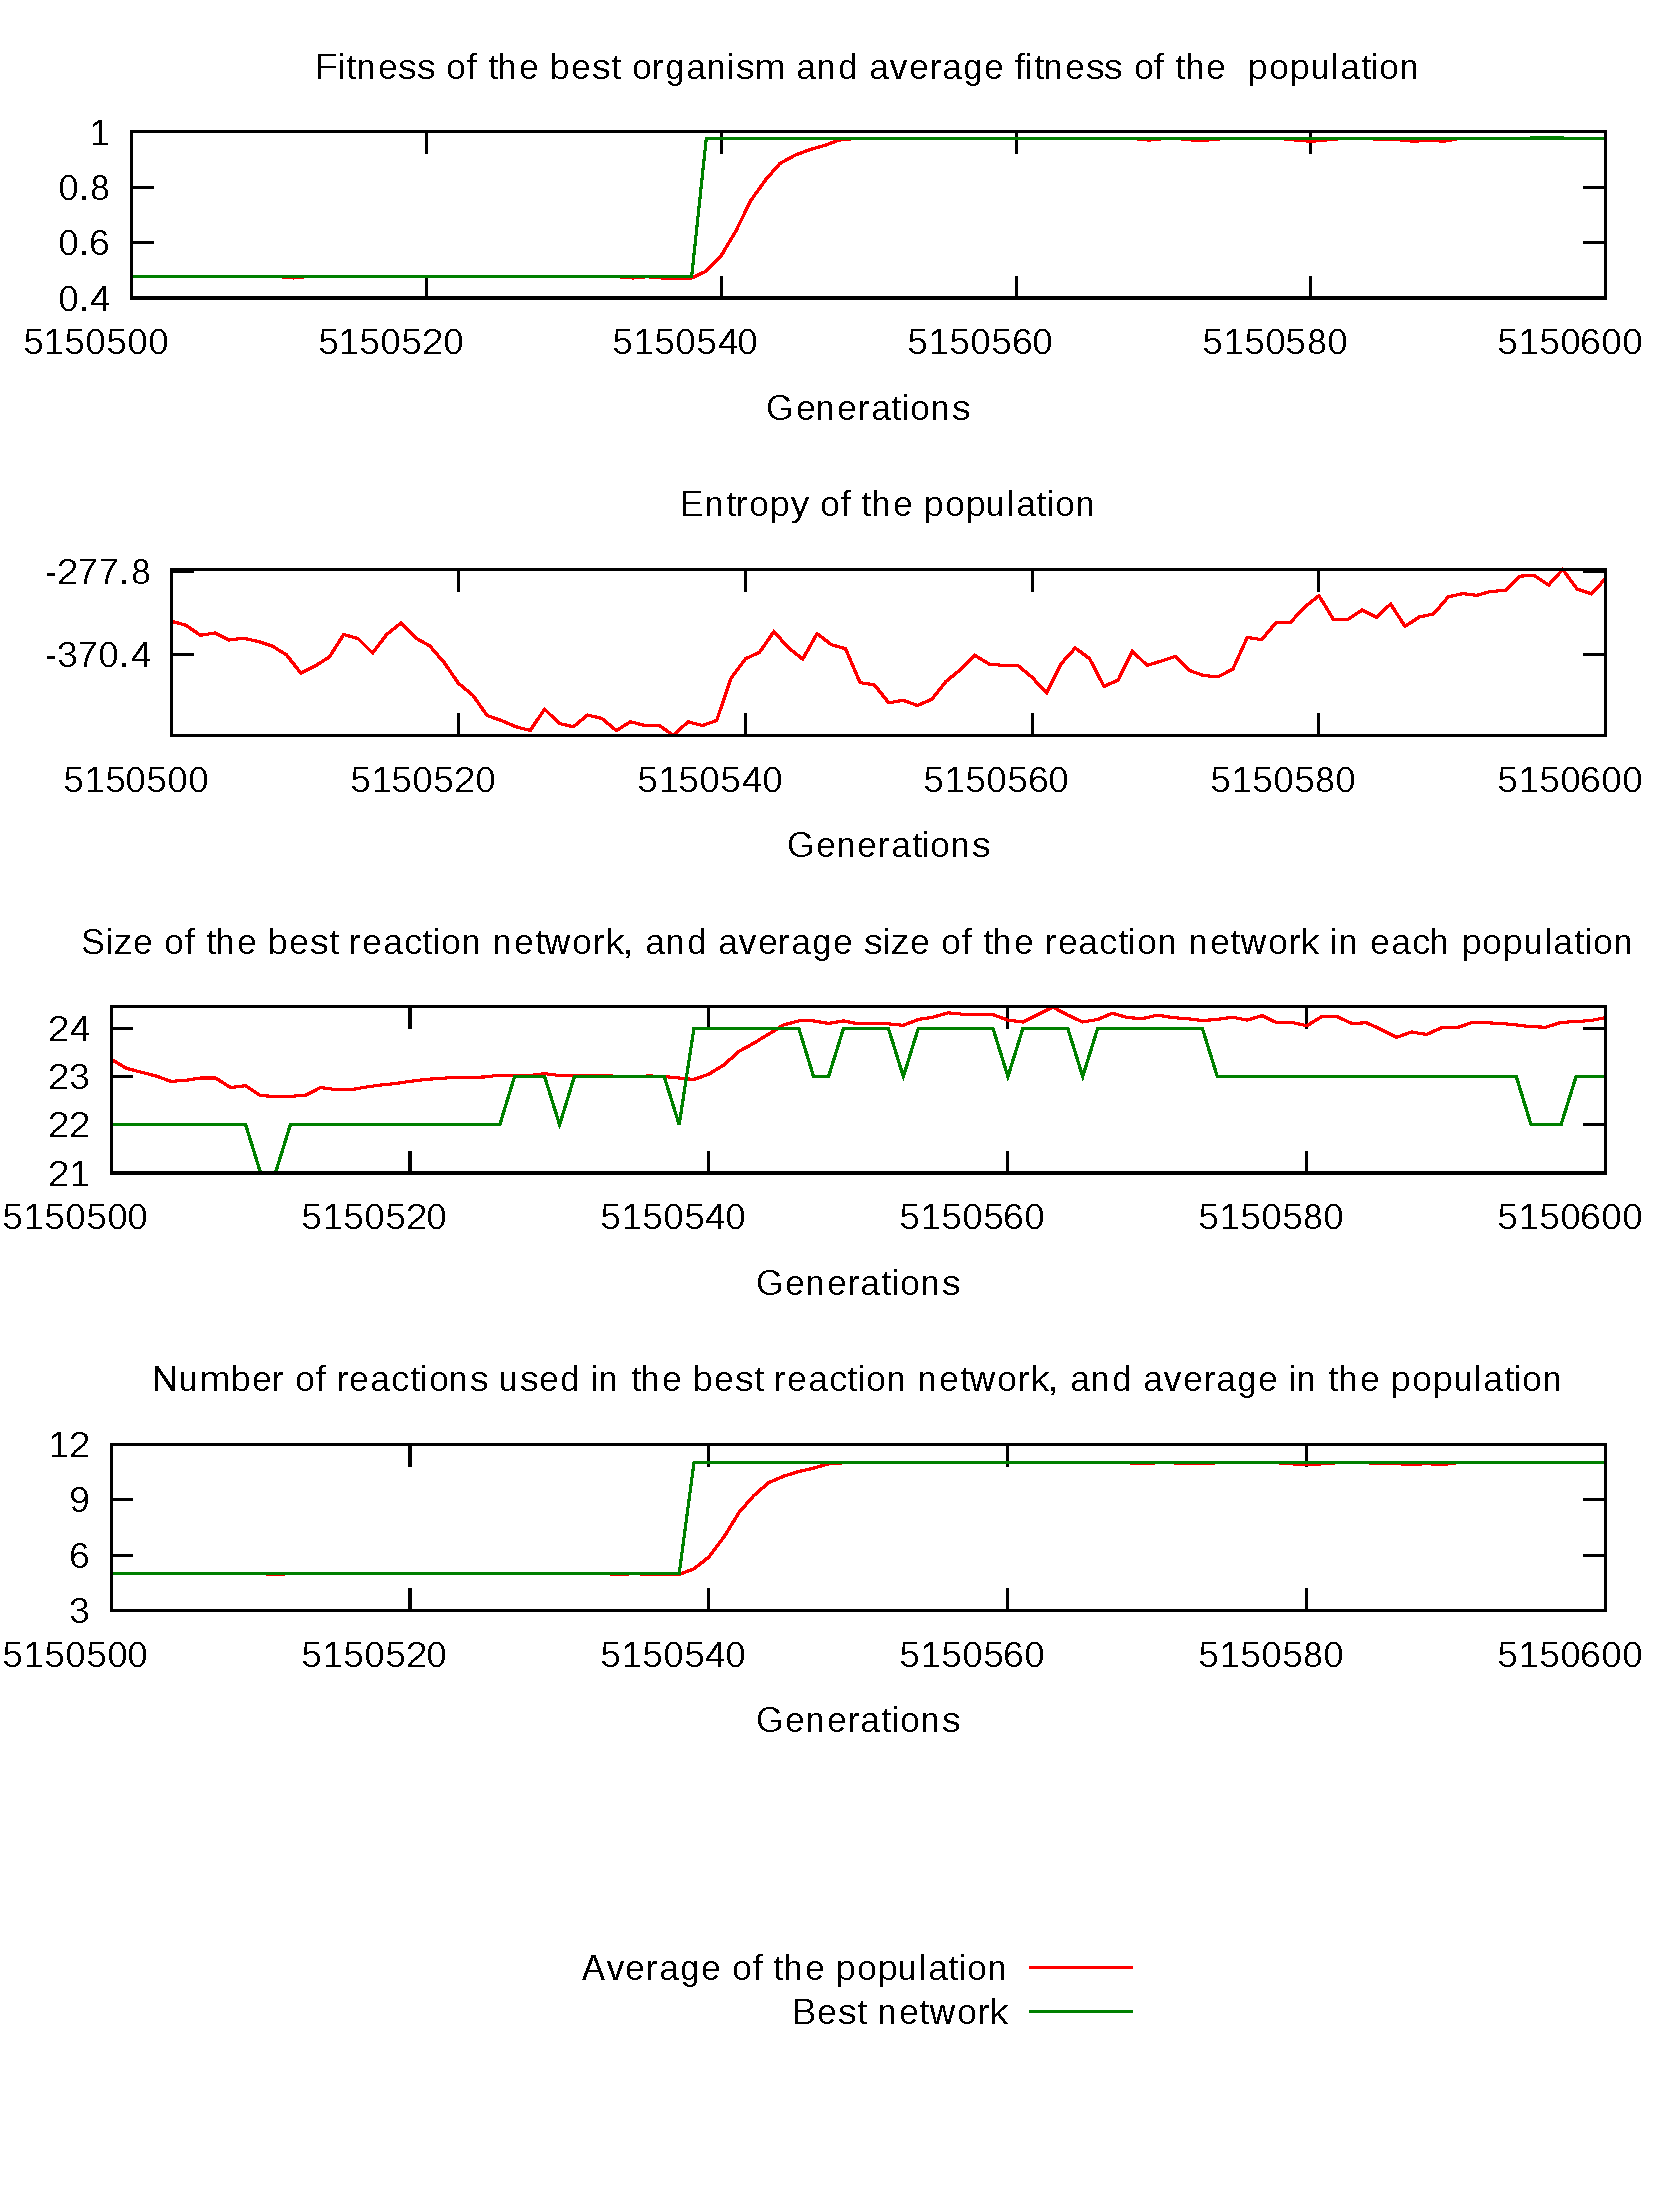
\includegraphics[width=0.8\linewidth]{fixation.pdf}
	\caption{Extract of summary statistics of Population 1 of Simulation 2 showing the fixation of a beneficial mutation}
	\label{fig:fixation}
\end{figure}

As such fixations remain invisible on a plot whose $x$ axis is on the order of $10^5-10^6$ such as Figure~\ref{fig:simulation1}, the first and second pair of graphs are very similar. In consequent diagrams we shall show only one graph of each pair (fitness, total number of reactions, and number of used reactions).

All populations in Simulation 1 have improved their fitness by increasing the ADP ATP conversion rate by $0.5$ or $1$. The times of improvements are distributed approximately uniformly and after any jump-improvement in all curves we can observe a slight decline in fitness. This phenomena is due to the MN-s gaining access to more and more reactions (of which few are only used), as can be seen on graphs 3 and 4 of Figure~\ref{fig:simulation1}. Observe that the increases in the number of reactions in the MN-s start to increase when the fitness increases. The number of used reactions (those with non-zero flux through them in the optimal steady state solution) are shown on the last pair of graphs on Figure~\ref{fig:simulation1}, for the best network and for the average network. The reaction network with ATP production of $0.5$ uses $\sim 6$ reactions, to produce $1$ ATP it needs $\sim 10$, and for $1.5$ ATP it needs $14$. 

The used reactions of the best performing network of Population 3 of Simulation 1 are shown on Figure~\ref{fig:trunk_glyc_final_job1}. The network found alternative pathways to bypass the restrictions imposed by the bounds on the reaction fluxes. The two longer alternative pathways (to the left) meet at phosphoenolpyruvate, and there they diverge again, one converting an previously produced AMP (adenosin monophosphate SPELLING?) to ATP while the other converting ADP to ATP. We observe similar meeting and diverging paths in the simulations that follow. In real glycolysis 3-phosphorglycerate is isomerized to 2-phosphorglycerate, this network therefore performs almost all reactions that real glycolysis does, but not in a single path. 



\begin{figure}[htpb]
	\centering
	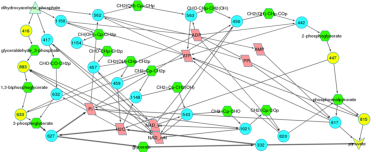
\includegraphics[width=1\linewidth]{trunk_glyc_final_job1_colored.pdf}
	\caption{Reactions with nonzero flux in the fittest network at the end of the Simulation 1 in Population 3. The reactions of real glycolysis have been coloured yellow. }
	\label{fig:trunk_glyc_final_job1}
\end{figure}

An overview of the MN-s is shown on Figure~\ref{fig:init-mid-final} at three points in time, the beginning of the simulation (left), at the midpoint, after $1.5 10^5$ generations, and the final stage. The disconnected nodes at the bottom of the left plot are yet unused internal metabolites. Note the small disconnected components of the middle and the left plots. These are a result of the mutation method implemented in our program, described in Section \ref{sub:implementing evolution}. 

\begin{figure}[htpb]
	\centering
	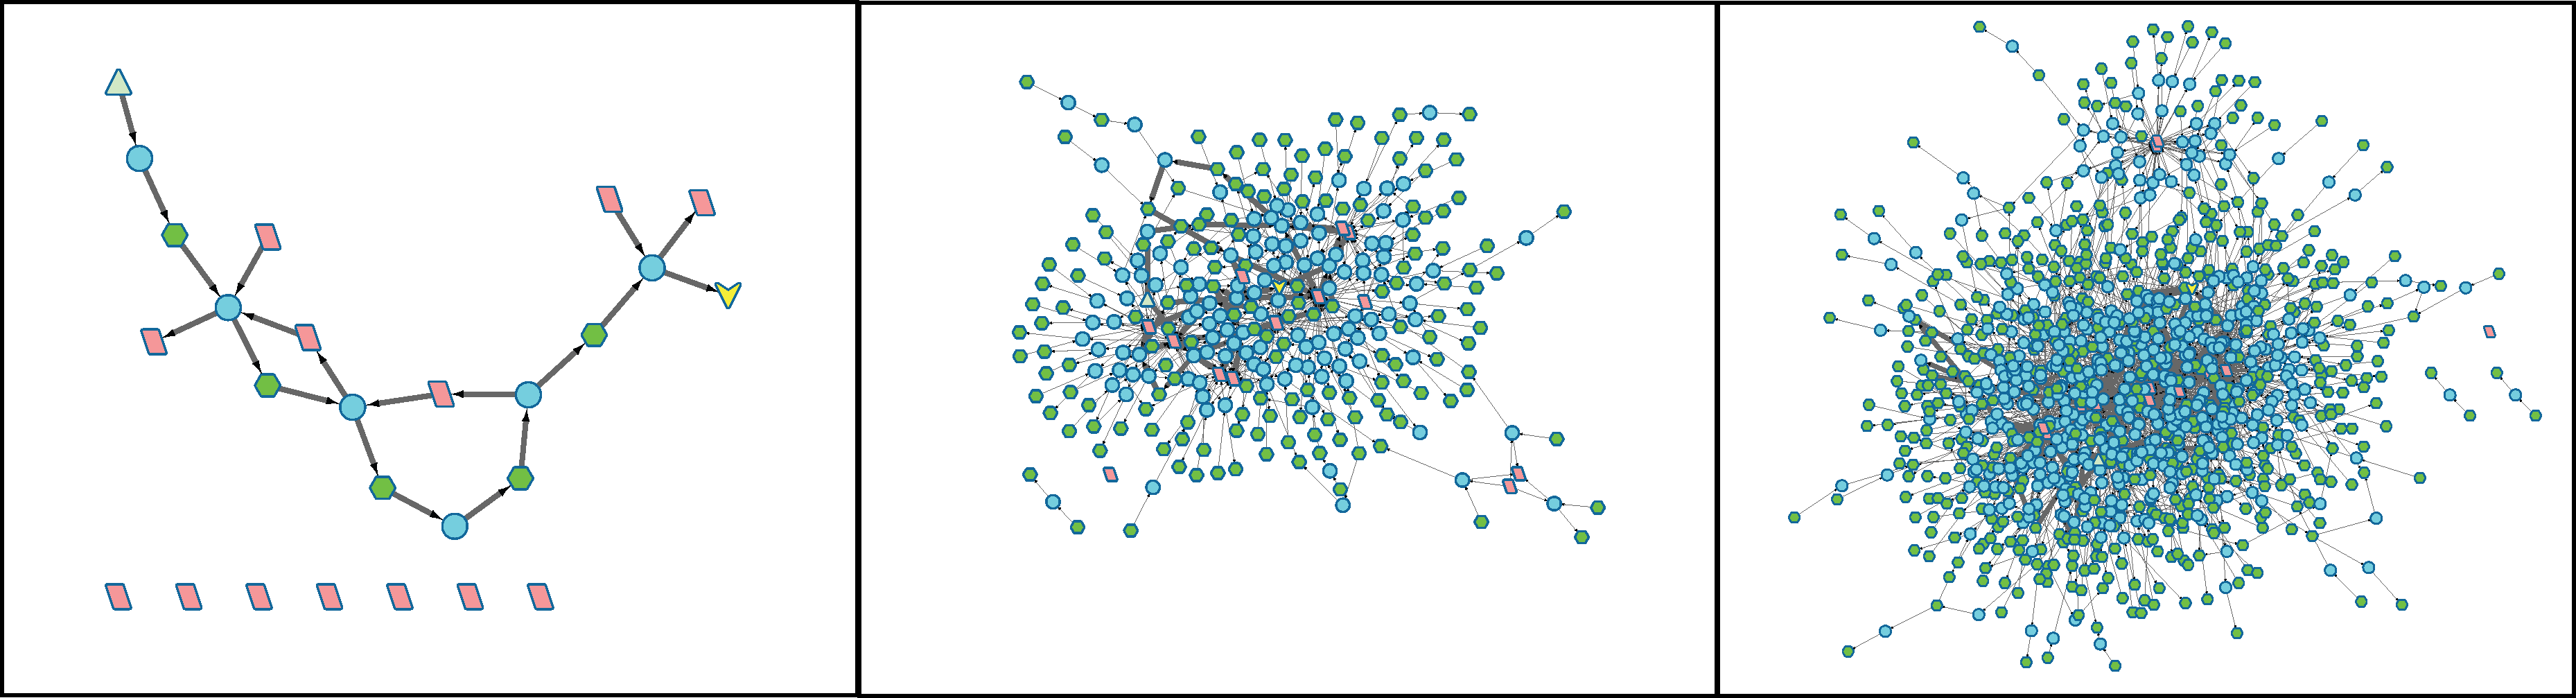
\includegraphics[width=1\linewidth]{init-mid-final.png}
	\caption{Overview of the best performing metabolic network of Population 3 of Simulation 1 at three stages of it's evolution, at the start of the simulation, at the midpoint, and at the end}
	\label{fig:init-mid-final}
\end{figure}

On the middle and left images of Figure~\ref{fig:init-mid-final} some nodes can be observed around which the network appears to be centered. To examine this we plot the node degree distribution of the final MN on Figure~\ref{fig:nodedegreedistro}. We find a small number of highly connected nodes (Hubs) and many less connected ones. One might call this a scale free network, therefore we fitted a power law distribution of the form $P(n)=n^{-\gamma}$, shown on Figure~\ref{fig:nodedegreedistro}. We found the parameter estimates to be $\gamma=1.236$. Similar distributions can be found when examining final networks of other simulations. 





\begin{figure}[htpb]
	\centering
	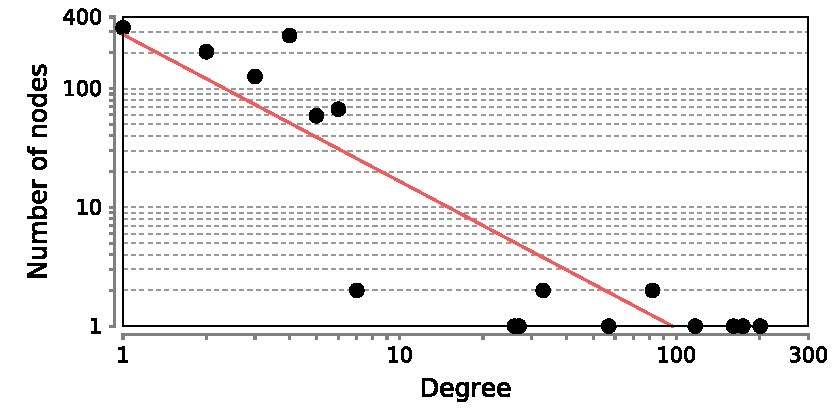
\includegraphics[width=0.8\linewidth]{nodedegreedistro.pdf}
	\caption{Node degree distribution of the final network of Population 3 of Simulation 1 with a power law distribution fitted}
	\label{fig:nodedegreedistro}
\end{figure}

\begin{figure}[htpb]
	\centering
	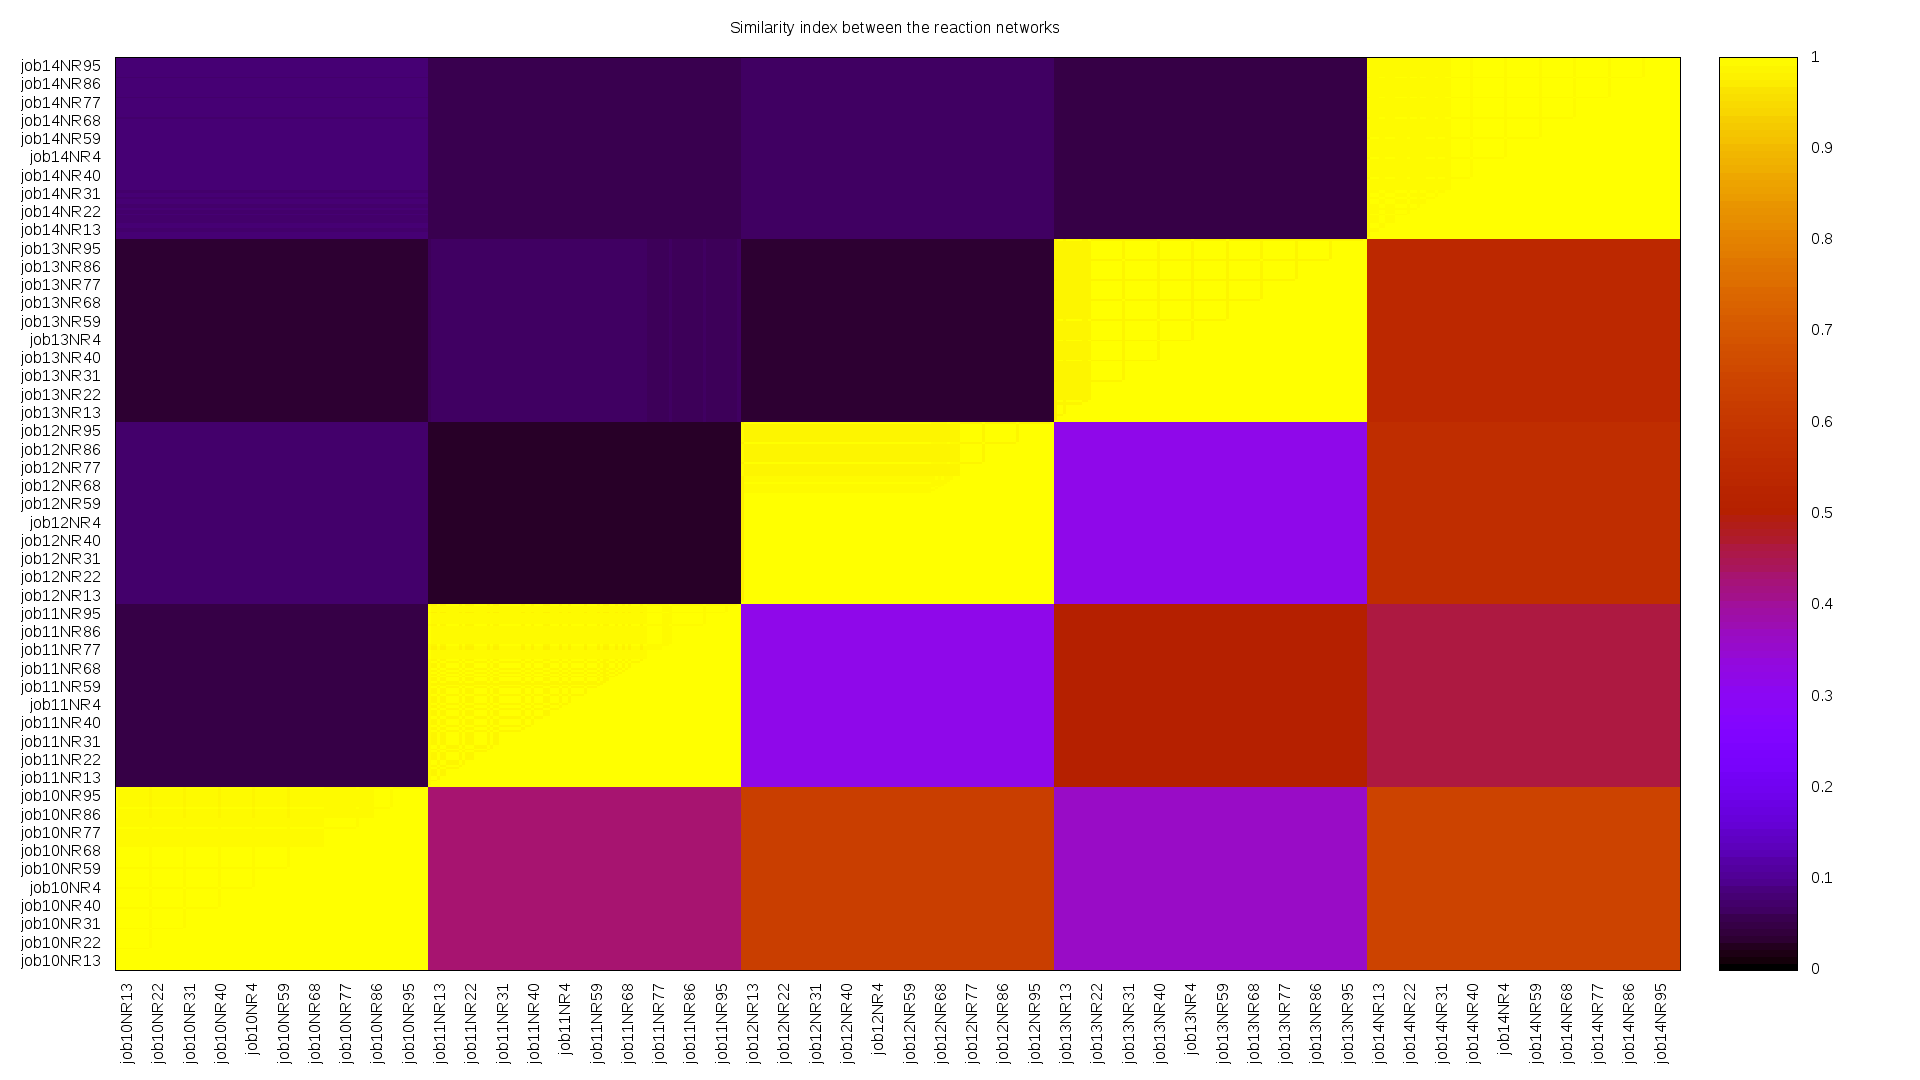
\includegraphics[width=1\linewidth]{simmatrix_firstjob.png}
	\caption{Similarity matrix of the first 3 populations of Simulation 1}
	\label{fig:simmatrix_firstjob}
\end{figure}

\subsection{examining The probability of the mutations}
\label{sub:the_probability_of_the_mutations}

The first pair of simulations were run to examine the effect of the mutation probability on the patterns of evolution. The initial MN and the goal function of these simulations was the same as for Simulation 1. The probability of point mutation was set to $p_{point}=0.01$ with the cost of reaction $k_{reaction}=0.001$ for Simulation 2, and for Simulation 3 $p_{point}=0.1$ with $k_{reac}=0.01$. The populations again consisted of $100$ cells each, giving the expected number of mutations per generation to be $1$ and $10$ for Simulations 2 and 3 respectively. 

Diagnostic plots for $3$ typical populations are shown on Figure~\ref{fig:simulation2} and Figure~\ref{fig:simulation3}.

Both simulations evolved the populations of MN-s for $6\times 10^7$ generations. This meant that Simulation 3 had 10 times more mutations than Simulation 2. 

Simulation 2 evolved the populations through approximately $600 000$ mutations, and of the populations completed the run $\sim 28 \%$ had no improvement in their fitness $\sim 55 \%$ had an improvement of $\sim 0.5$, and $16 \%$ have improved by $\sim 1$. The discovery of a new pathway to produce ATP increases the fitness function by $0.5$, but after such an improvement the MN-s usually GATHER a larger amount of unused reactions, in this case about $70$ reactions. This lowers the fitness function by $70 k_{reac}=0.07$. The number of unused reactions fluctuates WIDELY around $\sim 110$ for a network with fitness $\sim 1$, and around $\sim 150$ for a cell with fitness $\sim 1.4$. The number of reactions necessary for a fitness increase is $6$ ($11$ reactions in total), and the other increase could be achieved using an additional $4$ reactions ($15$ reactions in total). Thus only $\sim 10\%$ of the reactions are used within a MN.  The entropy of the population fluctuates around $\sim -360$ which can correspond to a population of $\sim 80$ identical cells, and a few mutants that are different from them. This can be observed on the similarity matrix of the final networks NOT SHOWN HERE

When visualizing the final networks of this simulation pathways similar to those at the end of Simulation 1 emerge. The networks have again "rediscovered" reaction $633$, and found alternative pathways to produce ATP. The alternative pathways are longer than the original glycolysis, and in the fittest networks they run in pairs. These pairs of pathways run from DHAP to pyruvate, but they meet at intermediate compounds, in some cases more than once. Sometimes we find one of these pathways not producing any net ATP, but they contribute to the other part of the pair by providing nutrients to it (eg. phosphate). When considering the node degree distribution of the resulting networks the results are similar to those shown on Figure~\ref{fig:nodedegreedistro}. 


\begin{figure}[htpb]
	\centering
	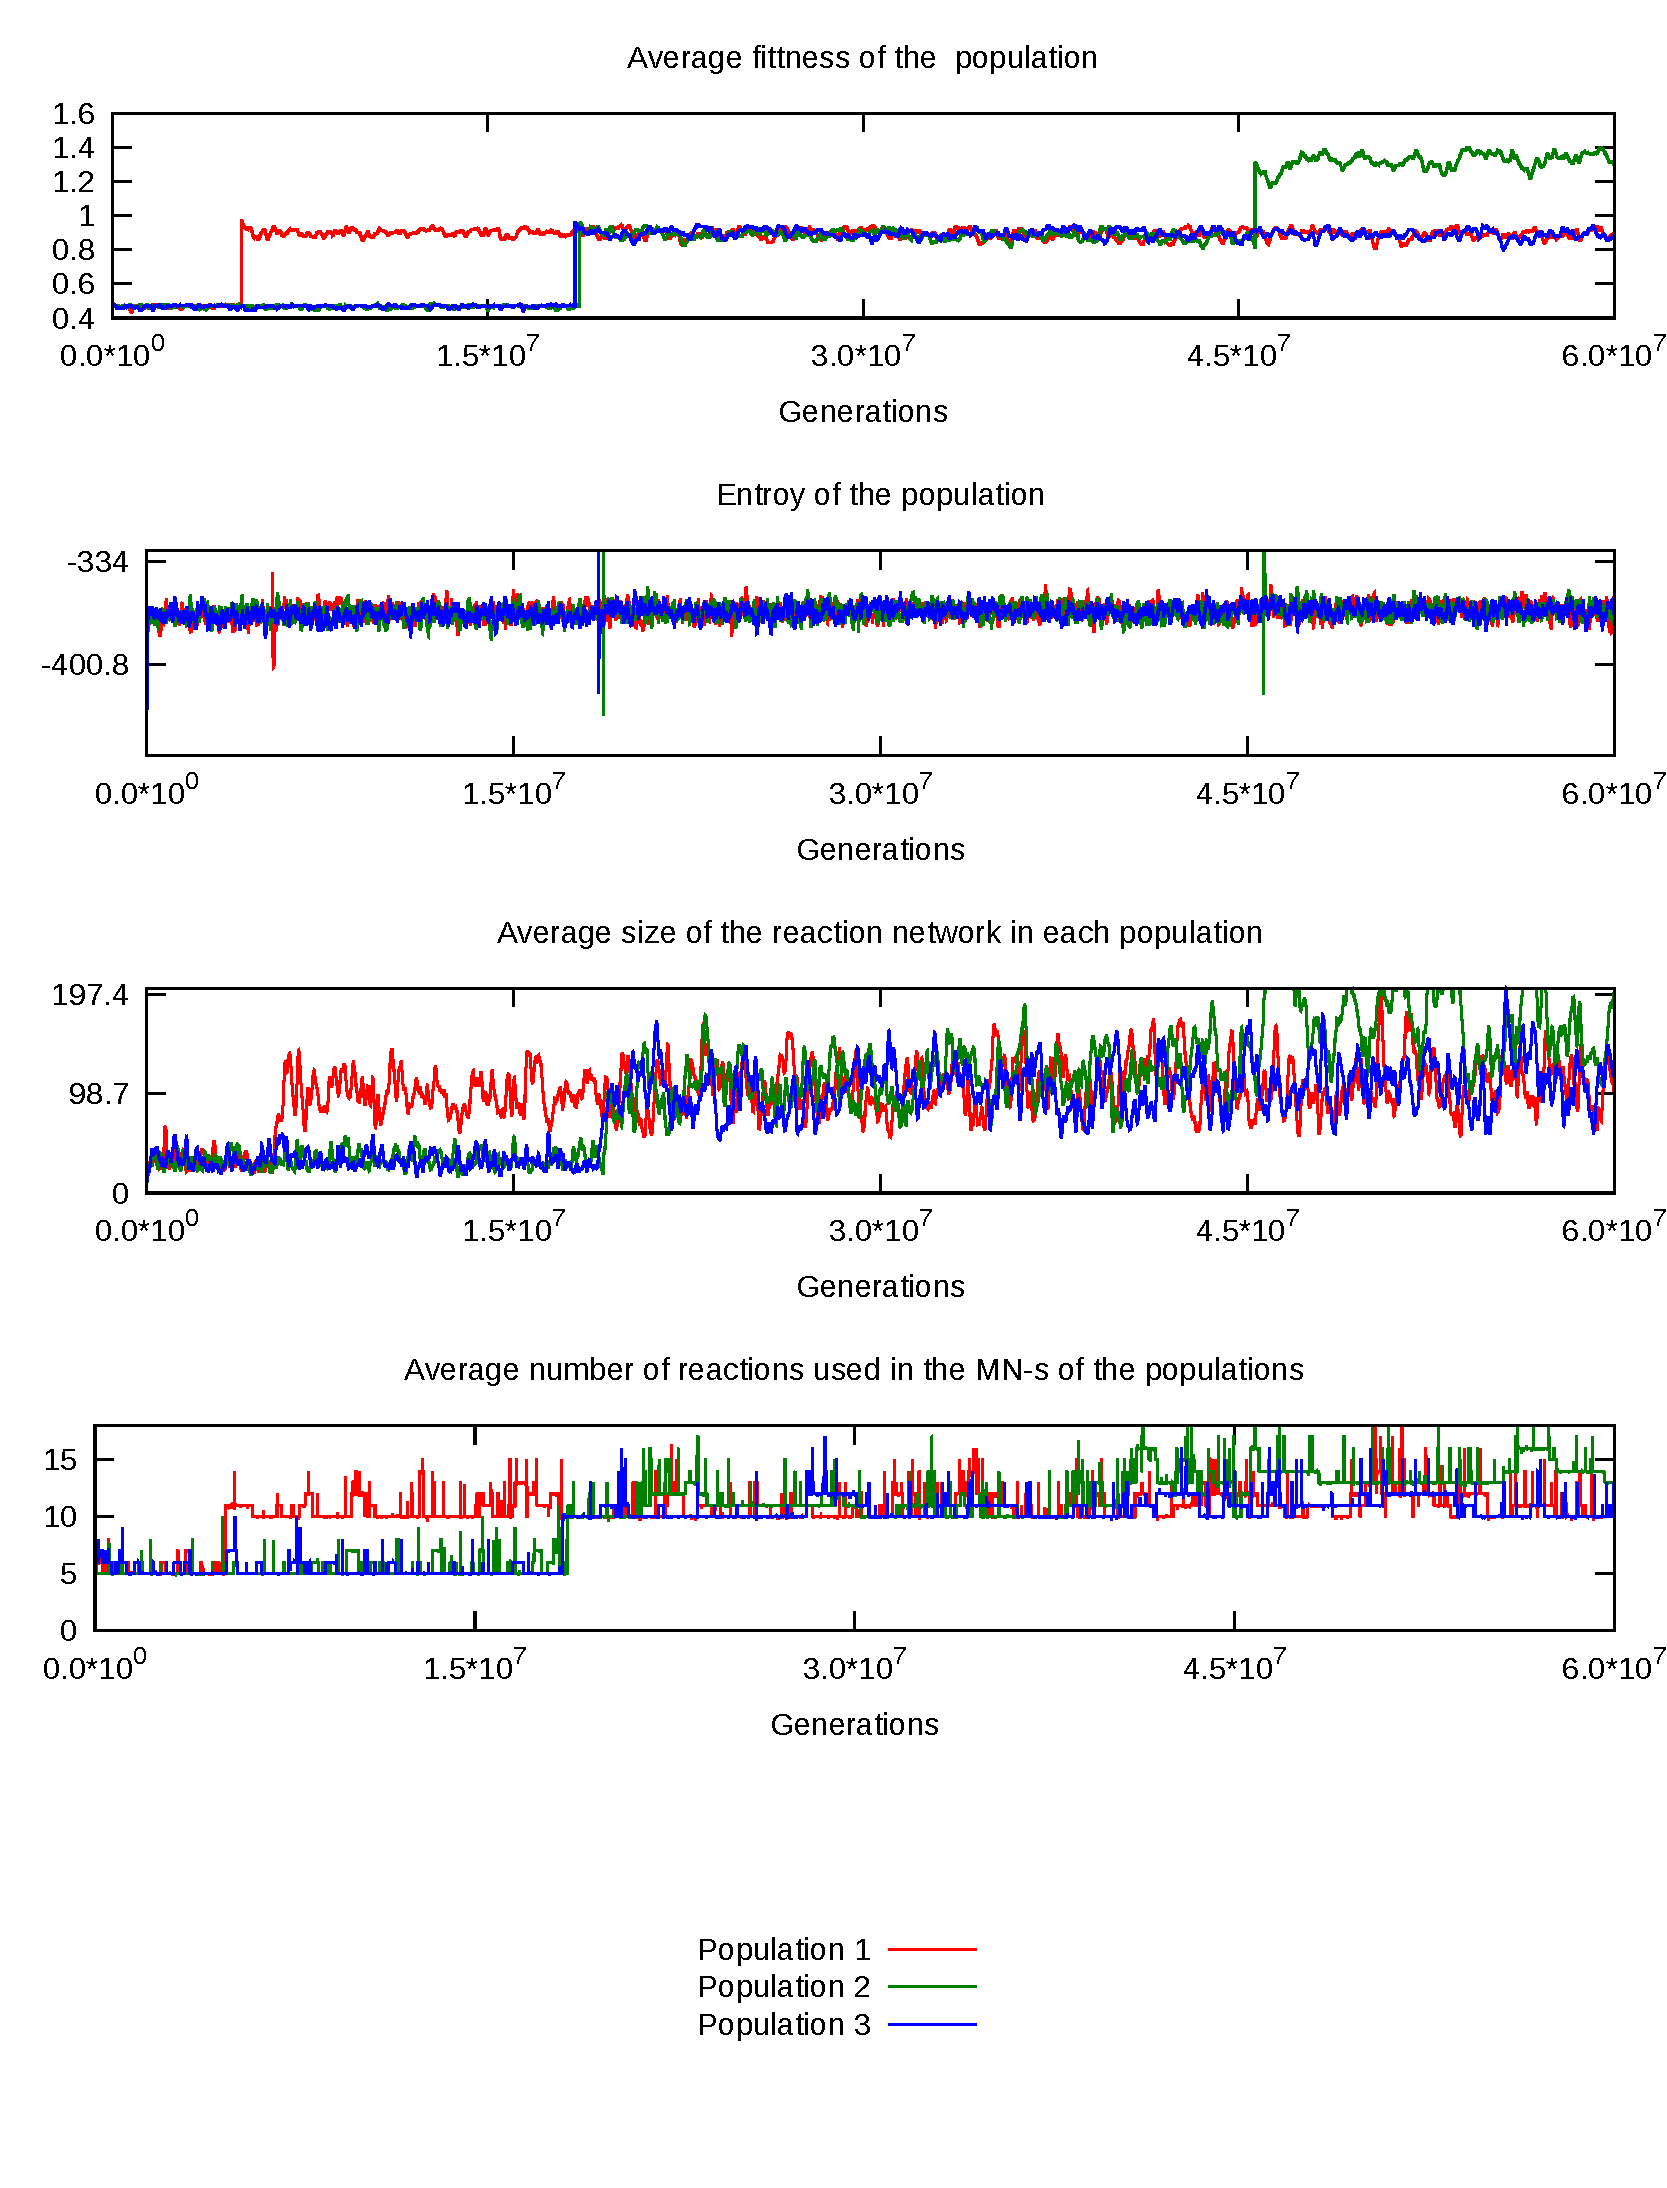
\includegraphics[width=0.8\linewidth]{simulation2.pdf}
	\caption{Diagnostic plots of 3 typical populations of Simulation 2 TAKE CARE OF ENTROY TYPO}
	\label{fig:simulation2}
\end{figure}

\begin{figure}[htpb]
	\centering
	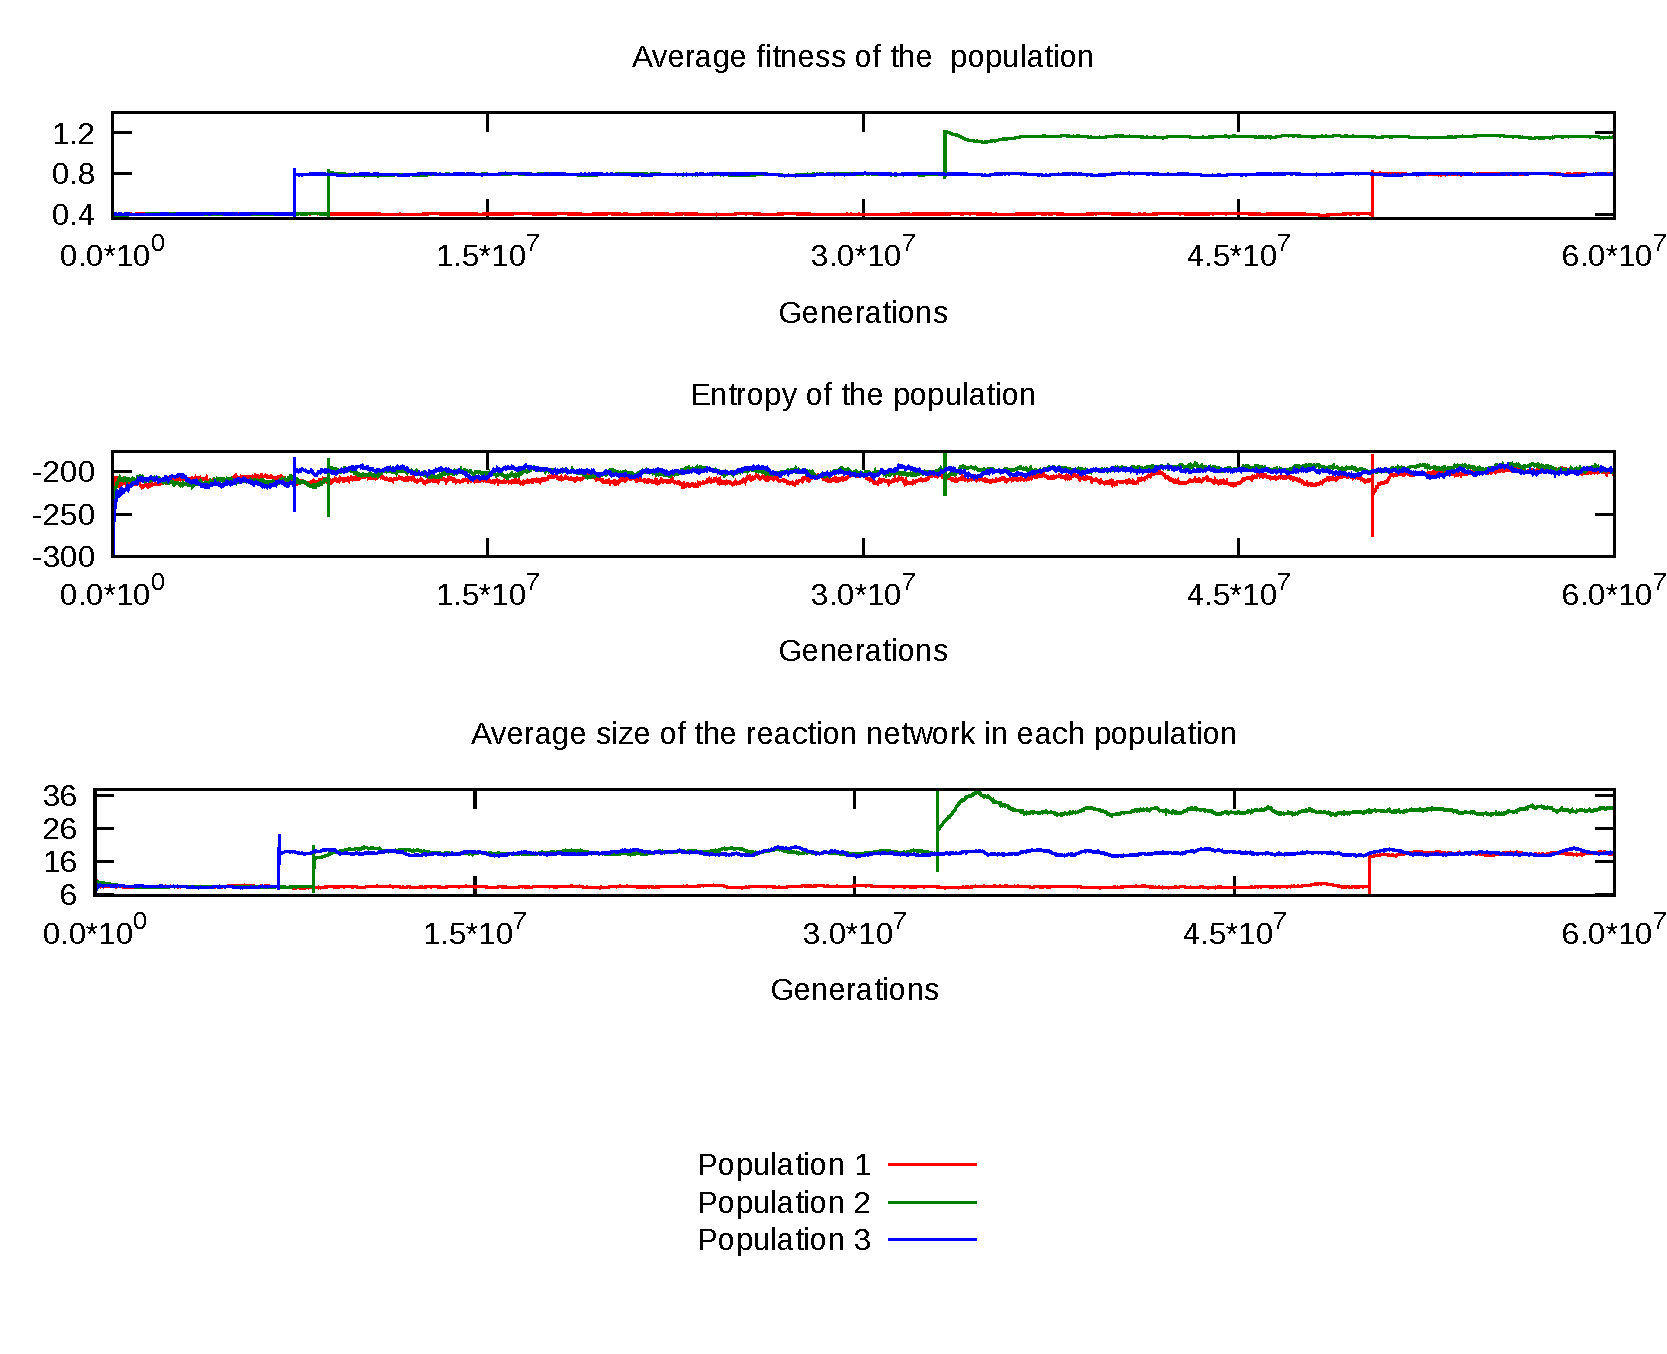
\includegraphics[width=0.8\linewidth]{simulation3.pdf}
	\caption{Diagnostic plots of 3 typical populations of Simulation 3 REMAKE THIS}
	\label{fig:simulation3}
\end{figure}

Simulation 3 had $10$ times more mutations than Simulation 2. Even though the number of reactions in the MN-s was smaller, due to a higher $k_{reac}$ value the populations of Simulation 3 improved further than those of Simulation 2. Here there were no simulations that did not improve, $\sim 16\%$ made $1$ improvement, $79\%$ made 2, and $5\%$ ($1$ population) made $3$ improvements in their ATP production. After an improvement the networks gain reactions here too, but they only gain $\sim 15$ networks after a single improvement. The total number of used reactions required for an improvement is similar to that of Simulation 2, but in this case the proportion of reactions used by the MN is $\sim 50\%$. The entropy of the populations fluctuates less wildly than that of Simulation 2, around $\sim -200$. This can correspond to $\sim 7$ approximately equal sized subpopulations, and a few lone mutants. This can be observed in the similarity matrix of the simulation shown on Figure~\ref{fig:simmatrix_sim3}. The used reactions are identical within almost every reaction within a population, and they show a rather large degree of similarity between populations too. When considering the whole metabolic network we can see that the populations themselves are diverse, but within a population networks only differ from each other by a handful of reactions. 

We also considered a simulation with $p_{point}=0.01$ and $k_{reac}=0.01$ but none of the 20 populations produced any improvement after a similar simulation time as used above. 


\begin{figure}[htpb]
	\centering
	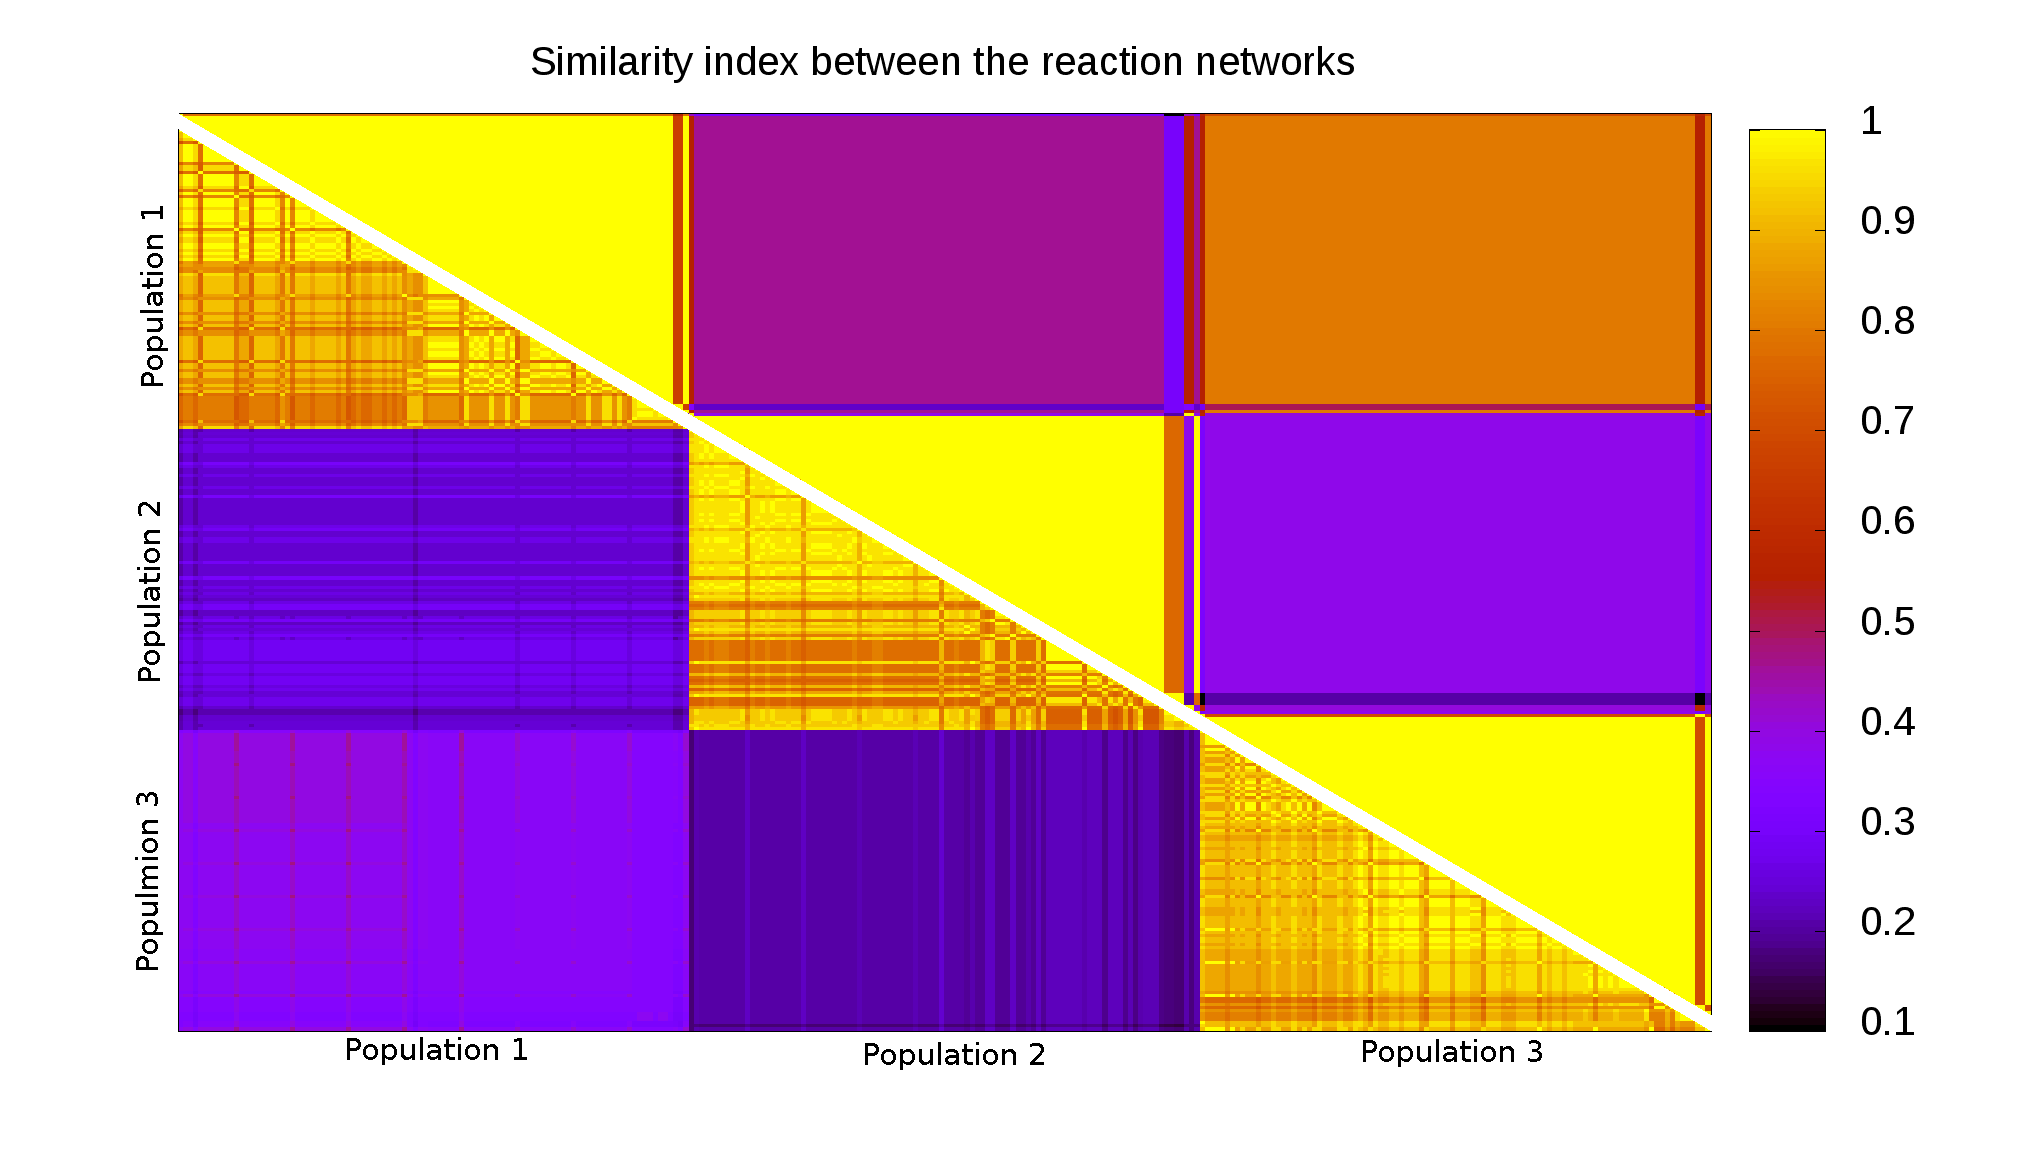
\includegraphics[width=0.8\linewidth]{simmatrix_sim3.png}
	\caption{Similarity matrix of 3 populations of Simulation 3. Similarity indices calculated for used reactions are shown above the diagonal, while those calculated for the whole MN are below the diagonal}
	\label{fig:simmatrix_sim3}
\end{figure}

The fittest network of Population 1 at the end of the simulation is shown on Figure~\ref{fig:trunk_glyc_final_job1}. This network uses parts of the original network (reactions $416$ and $883$ for the beginning of the path on the left of the figure, and reaction $633$ was "rediscovered" by the network. 

\begin{figure}[htpb]
	\centering
	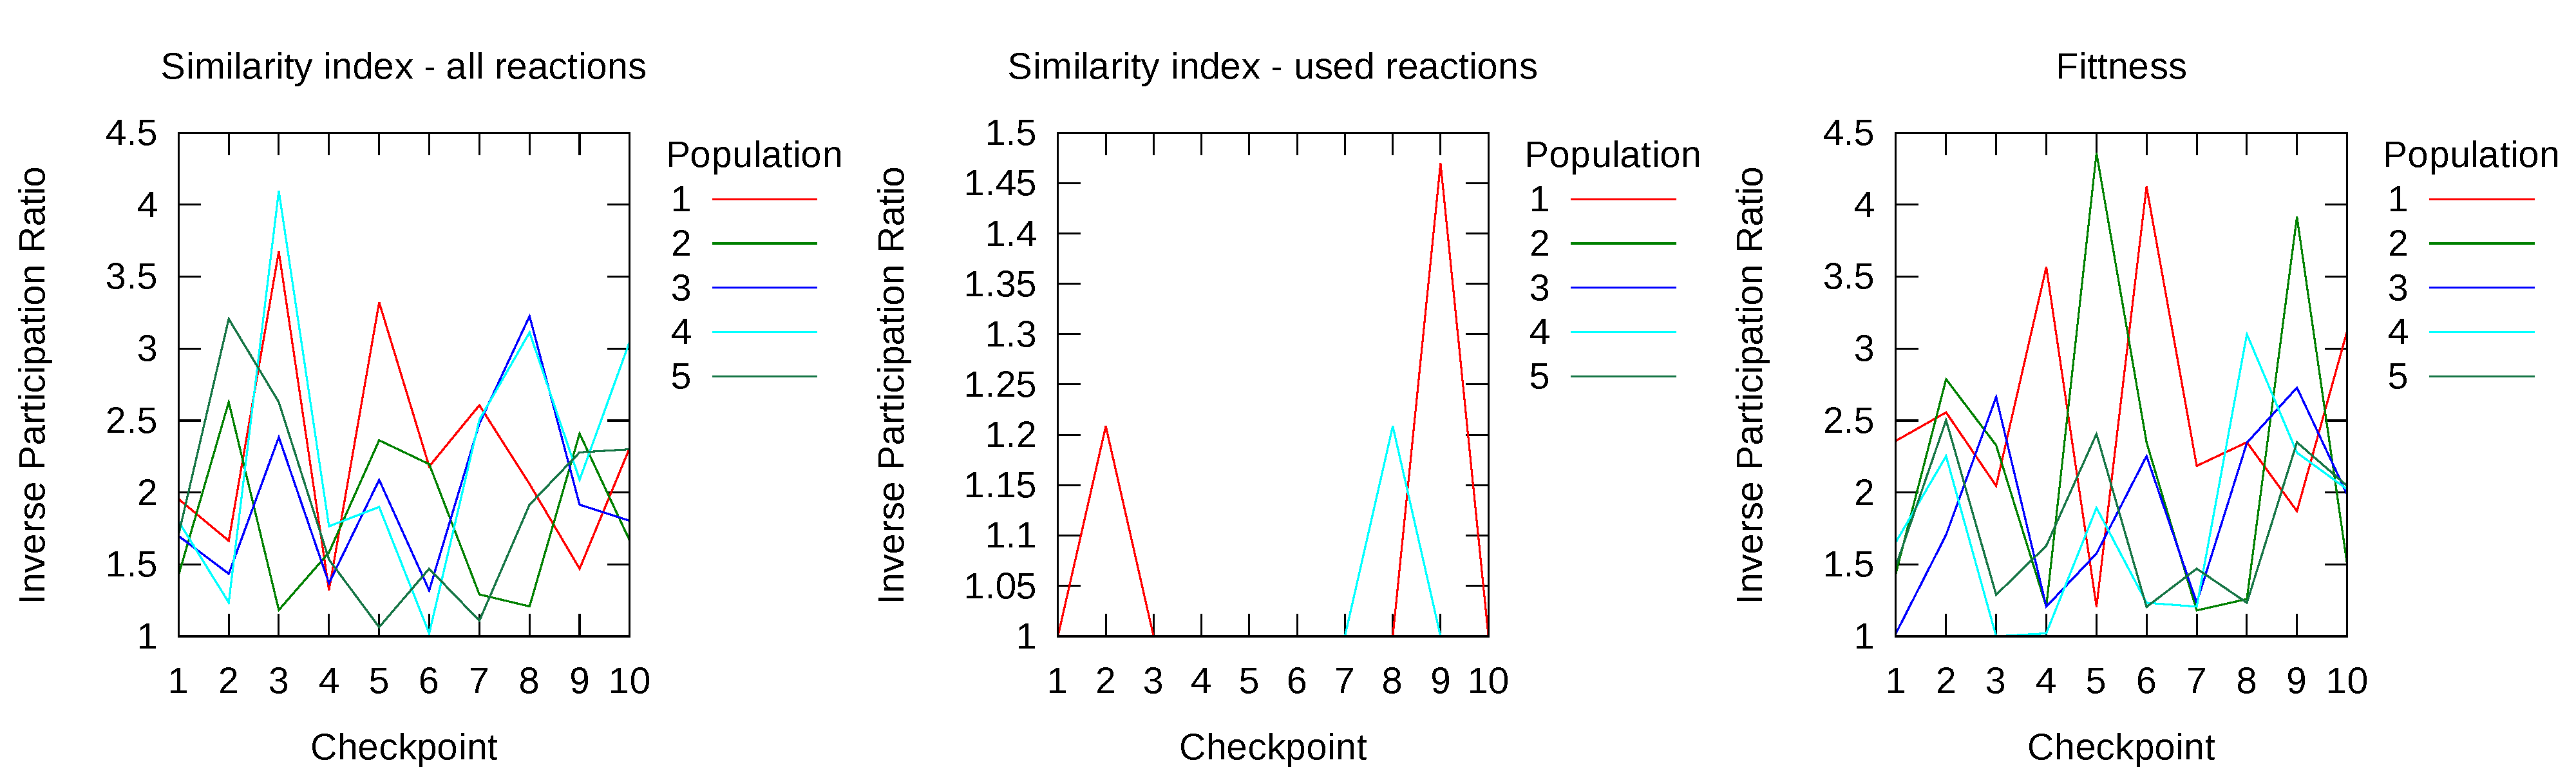
\includegraphics[width=1\linewidth]{IPR_longerlog.pdf}
	\caption{Inverse proportionality ratio plots of the first few populations}
	\label{fig:IPR_firstrun}
\end{figure}




The IPR plots of the first few populations are shown on Figure~\ref{fig:IPR_firstrun}, the plots of the not-shown populations are very similar to this one. The leftmost plot shows the IPR of the similarity indices of each cell compared to the best network. There is some variation in the reactions within the MN-s due to the random mutations, however when looking at the middle plot showing the IPR for the similarity indices calculated using the reactions with nonzero fluxes, there is very little variation. This is due to the fact that once a network evolves, there is generally only a small amount of minor changes can occur with the used reactions. 


The similarity indices for this simulation are shown on Figure~\ref{fig:simmatrix_firstjob}, for all the reactions in the MN-s above the diagonal, and for the reactions with nonzero flux below it. 


\subsection{Multiple sources and sinks}
\label{sub:multiple_sources_and_sinks}

Real cells import a variety of nutrients from their environment, and most of their MN-s can run on multiple similar compounds \cite{latent}. To test how the presence of multiple sources influences the process of evolution of our networks, we performed simulations of networks that had access to $2$ nutrients. To be able to compare the resulting networks with our previous simulations, the initial network was, as previously, the modified trunk of glcolysis, shown on Figure~\ref{fig:truncglycinit}. The two sources used for this network were DHAP as before, and G3P. These two molecules are the end products of the upper glycolytic pathway. They enter the lower part by DHAP being converted into G3P, and the two G3P molecules undergo the same trunk pathway. The sink of the simulation was Pyruvate, as before, with the goal function rewarding ATP production only. The simulation was run using $P_{point}=0.01$ and $k_{reac}=0.001$. We relaxed the condition on the flux of phosphate, allowing the cell to take phosphate up, or dispose of it. This allows the cell to remove phosphate by other means than the ADP $\rightarrow$ ATP conversion. Interestingly this was not used by the cells. We call this run Simulation 6 SIMNAMING!!!

\begin{figure}[htpb]
	\centering
	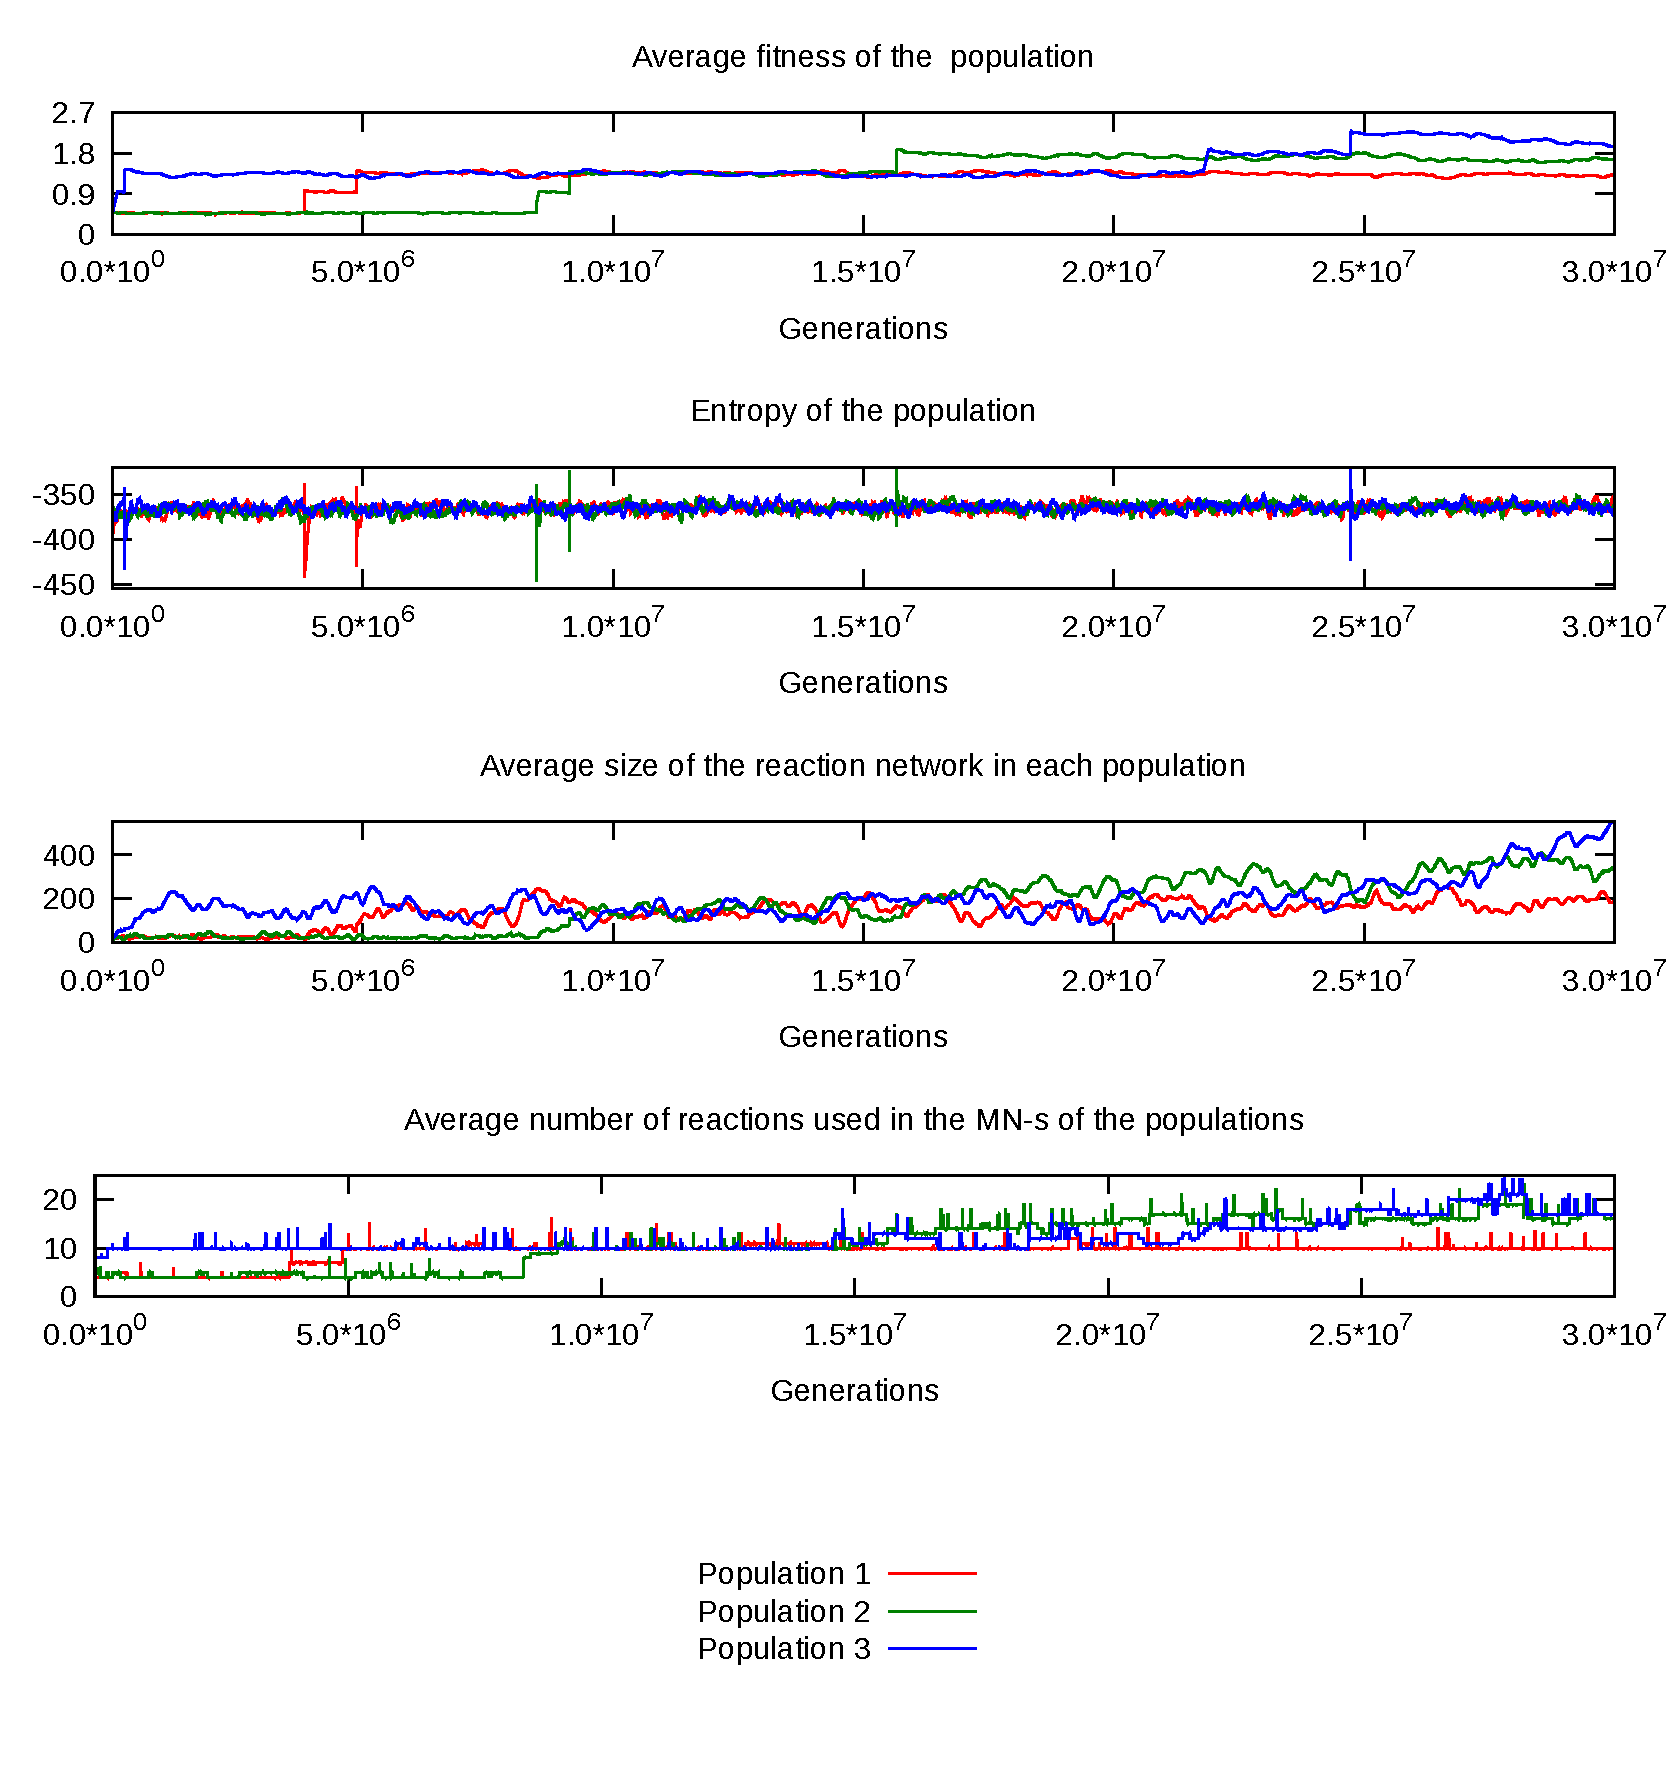
\includegraphics[width=1\linewidth]{simulationmultisource.pdf}
	\caption{Diagnostic plots for 3 populations of Simulation 6}
	\label{fig:simulationmultisource}
\end{figure}

Diagnostic plots for $3$ populations are shown on Figure~\ref{fig:simulationmultisource}. All of the populations that finished the simulation made at least $2$ improvements in their ATP production. These first two improvements appeared rather early in the simulation, with the last population to obtain them being Population~$2$. These two improvements increase the number of used reactions to $10$, and the networks acquire $\sim 200$ reactions in total.  Approximately $22\%$ of the simulations made $3$ improvements, and $11\%$ made $4$ improvements. The number of reactions necessary for the $3$ improvement network is $14$, and with $17$ reactions the system can produce $4$ improvements. The entropies of the populations are similar to the previous simulatinons. 



\begin{figure}[htpb]
	\centering
	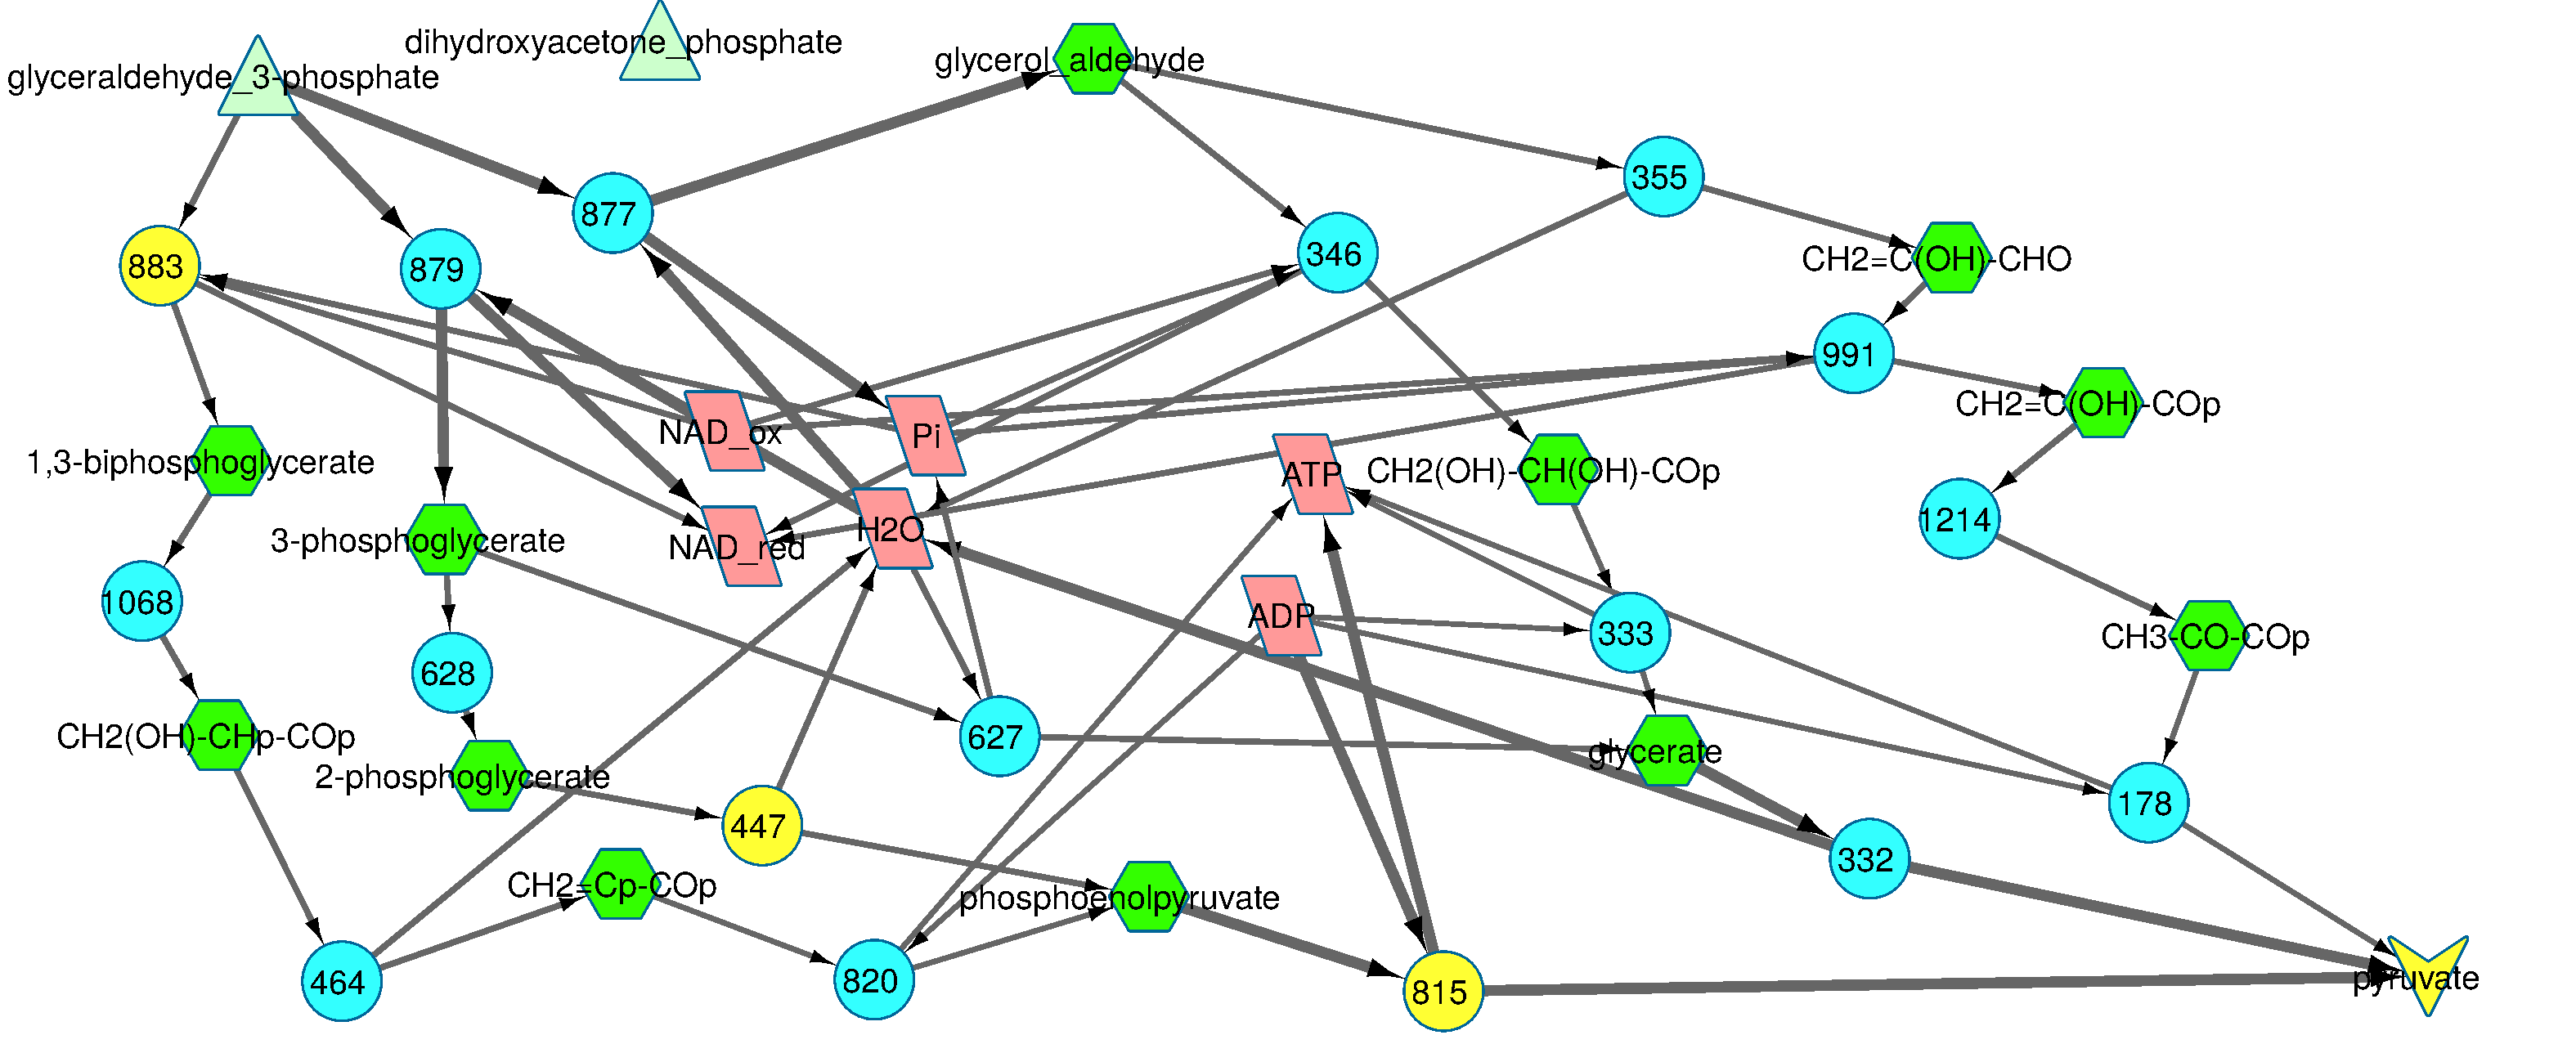
\includegraphics[width=1\linewidth]{multisink_finalnet.pdf}
	\caption{The best performing network at the end of Simulation 6. The reactions used by real glycolysis have been coloured yellow. }
	\label{fig:multi}
\end{figure}

We show one of the fittest networks at the end of this simulation on Figure~\ref{fig:multi}. The network has abandodned the DHAP source, instead using only G3P. This is a phenomena appearing in all the populations. The flux through the reactions is shown on the figure by the different thickness of the arrows. The thinner ones symbolize reactions with flux $0.5$, while the thick ones mean a flux of $1$. It is important to note how interlinked the network is.  While there are 3 pathways leading away from G3P, and there are also $3$ leading in to pyruvate, these pathways are very connected. The pathways starting with reaction $883$ meets with the one starting with $879$ at phosphoenolpyruvate. Also the paths starting with $879$ and $877$ DIVIDE? DIVERGE? and meet at glycerate. 

When comparing the similarity matrices of the populations we find that the diversity within a population is small, much like on Figure~\ref{fig:simmatrix_sim3}. The networks with $3$ improvements show a large degree of similarity in the used reactions $\sim 0.8$. Of those with only $2$ improvements, there is a pair where the used reactions are identical, and many of them have a a moderate amount of similarity between them $\sim 0.6$. If we look at the whole list of reactions, any pair of networks show a very small degree of similarity $\sim 0.1-0.2$. This is expected, as the unused reactions are more or less random. 

\subsection{Similar networks reached in parallel runs}
\label{sub:similar_networks_reached_in_paralell_runs}
If mutations happen with 100$\%$ then rather fast improvement to best network. Very diverse populations in terms of available reactions, but somewhat similar within a single run. Different runs very different available reactions. For the nonzero flux reactions within a run is almost completely homogeneous, and lots of similarity between runs too. 

If the mutation probabilities decrease improvements become more difficult. 
\subsection{Changing nutrients of the network}
\label{sub:changing_nutrients_of_the_network}

\subsection{Multiple output (possibly changing)}
\label{sub:multiple_output_possibly_changing_}

\subsection{Horizontal gene transfer}
\label{sub:horizontal_gene_transfer}


\subsection{Limitations}
\label{sub:limitations}
Dynamics of chemical reactions ignored

Restrictions in the types of mutations

Small interactions between cells

Too simple goal function



\section{Discussion}
\label{sec:discussion}
\textbf{Small population, graph of network at 3 times}

In this work we have considered the effects of the rate of mutation and the goal function on the patterns of evolution in our model. 

\textbf{Discussion of probability examination results}
The authors of \cite{predictability} note that crucial parameters for modeling evolution, such as the frequency of beneficial mutations are not known. 

The main limitations of our model are due to the small population size, the restrictions on the chemistry and the simplifications introduced by using flux balance analysis. 

The populations of simple organisms, that our MN-s model are usually substantial. A $1$ ml liquid sample of bacterial colonies can contain bacteria in excess of $10^9$ \cite{barteklecture}. The probability of the fixation of a neutral mutation is inversely proportional to the population size, thus for such large populations it is very unlikely. In our populations with size $N=100$ approximately one in every hundred mutations fix in the population. This aides the emergence of beneficial mutations, since only a set of unused reactions can contribute to a fitness advantage. For example in Simulation 2 the MN-s need 4 additional reaction to produce more ATP. $3$ of these reactions must fix in the population as a neutral one, and stay dormant until the last reaction can fix too. Note that the disappearance of one of the $3$ unused reactions constitutes a neutral mutation too, therefore the disappearance of a reaction that could later be useful is also possible.

Although we have not examined the effect of population size in our model the program could easily be extended to accommodate a larger population. Existing research suggests that in case of larger populations the patterns of evolution become more deterministic with larger populations \cite{predictability}

	\textbf{About FBA, need more}
	This method is computationally fast and easy to implement, however it disregards most of the thermodynamic and chemical constraints on the speed of the reactions. By using it we make the assumption that all reactions happen at equal speeds, given the reactants are present the reaction will happen, and the direction of a reaction is defined by the free energy change at the specific conditions. It doesn't take into account the free energy landscape of the reaction, whether an energy barrier is blocking the reaction etc. (partially duplicate from section \ref{chap:whereisphysics}). The disregard of the energy barriers is justified by considering the cell's ability to lower such barriers using catalyst enzymes.

\bibliography{dissertation}
\bibliographystyle{plainnat}

\end{document}
